\documentclass[a4paper]{article}
\usepackage[14pt]{extsizes} 
\usepackage[T2A]{fontenc}
\usepackage[utf8]{inputenc}
\usepackage{natbib}
\usepackage{graphicx}
\usepackage{amsmath}
\usepackage[english, russian]{babel}
\usepackage{amsmath,amsfonts,amssymb,amsthm,mathtools,mathrsfs}
\usepackage{icomma}
\usepackage{fullpage}
\usepackage{ulem}
\usepackage{eufrak}
\usepackage{setspace}
\usepackage{listings}
\usepackage{indentfirst}
\usepackage[left=2cm,right=1.5cm,top=2cm,bottom=2cm]{geometry}
\usepackage{xcolor}
\usepackage{float}
\usepackage{csquotes}

\setlength{\parindent}{5ex}
\setlength{\parskip}{1em}
\renewcommand{\baselinestretch}{1}

\graphicspath{{images/}}

\definecolor{buzzlightyear}{HTML}{8757A5}
\definecolor{grass}{HTML}{738D06}
\definecolor{literal}{HTML}{F18A2B}
\definecolor{commentcolor}{HTML}{8E908B}

\lstdefinestyle{habrstyle}{
    backgroundcolor=\color{white},   
    commentstyle=\color{commentcolor},
    keywordstyle=\bfseries\color{buzzlightyear},
    numberstyle=\tiny\color{commentcolor},
    stringstyle=\color{grass},
    basicstyle=\ttfamily\footnotesize,
    breakatwhitespace=false,         
    breaklines=true,                 
    captionpos=b,                    
    keepspaces=true,                 
    numbers=left,                    
    numbersep=5pt,                  
    showspaces=false,                
    showstringspaces=false,
    showtabs=false,                  
    tabsize=4
}

\lstset{style=habrstyle}

\begin{document}
    % НАЧАЛО ТИТУЛЬНОГО ЛИСТА
    \begin{center}
        \begin{center}
        \hfill \break
        \normalsize{Санкт-Петербургский государственный политехнический}\\
        \normalsize{университет Петра Великого}\\
        \hfill \break
        \normalsize{\textbf{Высшая школа интеллектуальных систем и}}\\ 
        \normalsize{\textbf{суперкомпьютерных технологий}}\\ 
        \hfill \break
        \hfill \break
        \hfill \break
        \normalsize{Лабораторная работа №12}\\
        \hfill \break
        \hfill \break
        \normalsize{\LARGE GNU Radio}\\
        \end{center}
        \hfill \break
        \hfill \break
        \hfill \break
        \hfill \break
        \hfill \break
        \hfill \break
        \hfill \break
        \hfill \break
        \hfill \break
        \hfill \break
        \begin{flushright}
            \normalsize{Выполнил студент 3-го курса}\\
            \normalsize{группа 3530901/80201}\\
            \normalsize{Матвеец Андрей Вадимович}\\
            \hfill \break
            \normalsize{Преподаватель:}\\
            \normalsize{Богач Наталья Владимировна}\\
        \end{flushright}
        \hfill \break
        \hfill \break
        \hfill \break
        \hfill \break
        \begin{center} Санкт-Петербург\end{center}
        \begin{center}2021\end{center} 
        \thispagestyle{empty}
    \end{center}
    % КОНЕЦ ТИТУЛЬНОГО ЛИСТА
    
    % ОГЛАВЛЕНИЕ
    \newpage
        \tableofcontents
    
    % СПИСОК ИЛЛЮСТРАЦИЙ
    \newpage
         \listoffigures 
         
    \newpage
        \section{Постановка задачи}
            В данной лабораторной работе нам необходимо для начала обнаружить причины искажения сигнала и проблемы эффектов канала, после чего распознать этапы, которые будут необходимы для восстановления сигналов, а именно:
            
            \begin{itemize}
                \item Сроки восстановления
                \item Многолучевые каналы
                \item Фазовая и частотная корреляция
                \item Декодирования символов и упорядочение блоков
            \end{itemize}
            
            Помимо перечисленного необходимо разработать передатчик и приемник сигнала с  использованием квардратурной фозовой манимуляции средствами \texttt{GNU Radio}, и рассмотреть этапы с использованием алгоритмов уже доступных в \texttt{GNU Radio} для приема и демодуляции сигнала с реализацией фазовой манипуляции.
            
    \newpage
        \section{Часть №1: Передача сигнала}
           В первой части лабораторной работы нам необходимо создать квадратурную фазовую манипуляцию и передачу модифицированного сигнала. Генерируется сигнал (случайный поток битов), после чего он моделируется в сложное созвездие. Используется блок \texttt{Constellation Modulator}, который принимает объект \texttt{Constellation} и применяет различные настройки для управления передаваемым сигналом. Объект созвездия позволяет определить, каким образом кодируются символы. Модулятор \texttt{Constellation} использует фильтр формирования импульсов \texttt{RRC (root raised cosine)}, который предоставляет единственный параметр для настройки коэффициента спада фильтра - «альфа».
           
           Полученная диаграмма передает созвездие QPSK. Он строит как переданный сигнал, так и часть цепи приемника во времени, частоте и графике созвездия. Также стоит отметить, что имеются 3 ограничения: сигнал обязан укладываться в выделенную ему полосу пропускания. Передаваемые символы должны быть различимы. И, наконец, даже, если канал передачи не наложит значительных искажений, от шума все-равно не избавиться, поэтому передача сигнала должна обеспечивать хорошее соотношение сигнал/шум.
           
           \begin{figure}[H]
                \centering
                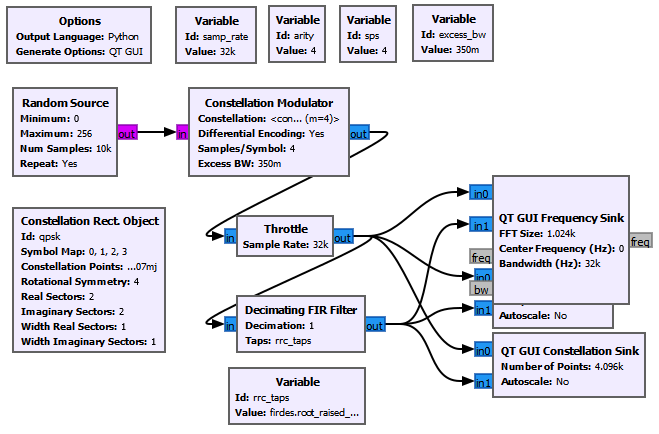
\includegraphics[width=\textwidth]{ex_1_1.png}
                \caption{Передача созвездия \texttt{QPSK}}
                \label{fig:ex_1_1}
            \end{figure}
            
            Ниже представлен график, демонстрирующий характеристики сигнала в “канале передачи” и на приемнике. 
            
            На графике \texttt{Constellation} виден эффект повышения частоты дискретизации и фильтрации. В этом случае фильтр RRC добавляет собственные помехи, известные как межсимвольные помехи (ISI). ISI не является подходящим для принятого сигнала, потому что он размывает символы. Если посмотреть на передаваемые сигналы с данного графика, можно видеть, что частотный график показывает сигнал с хорошей формой, который скатывается в шум. Если бы формирующий фильтр не был установлен на сигнал, передавались бы прямоугольные волны, которые производят много энергии в соседних каналах. Благодаря уменьшению внеполосных излучений сигнал остается в пределах полосы пропускания канала.
            
            \begin{figure}[H]
                \centering
                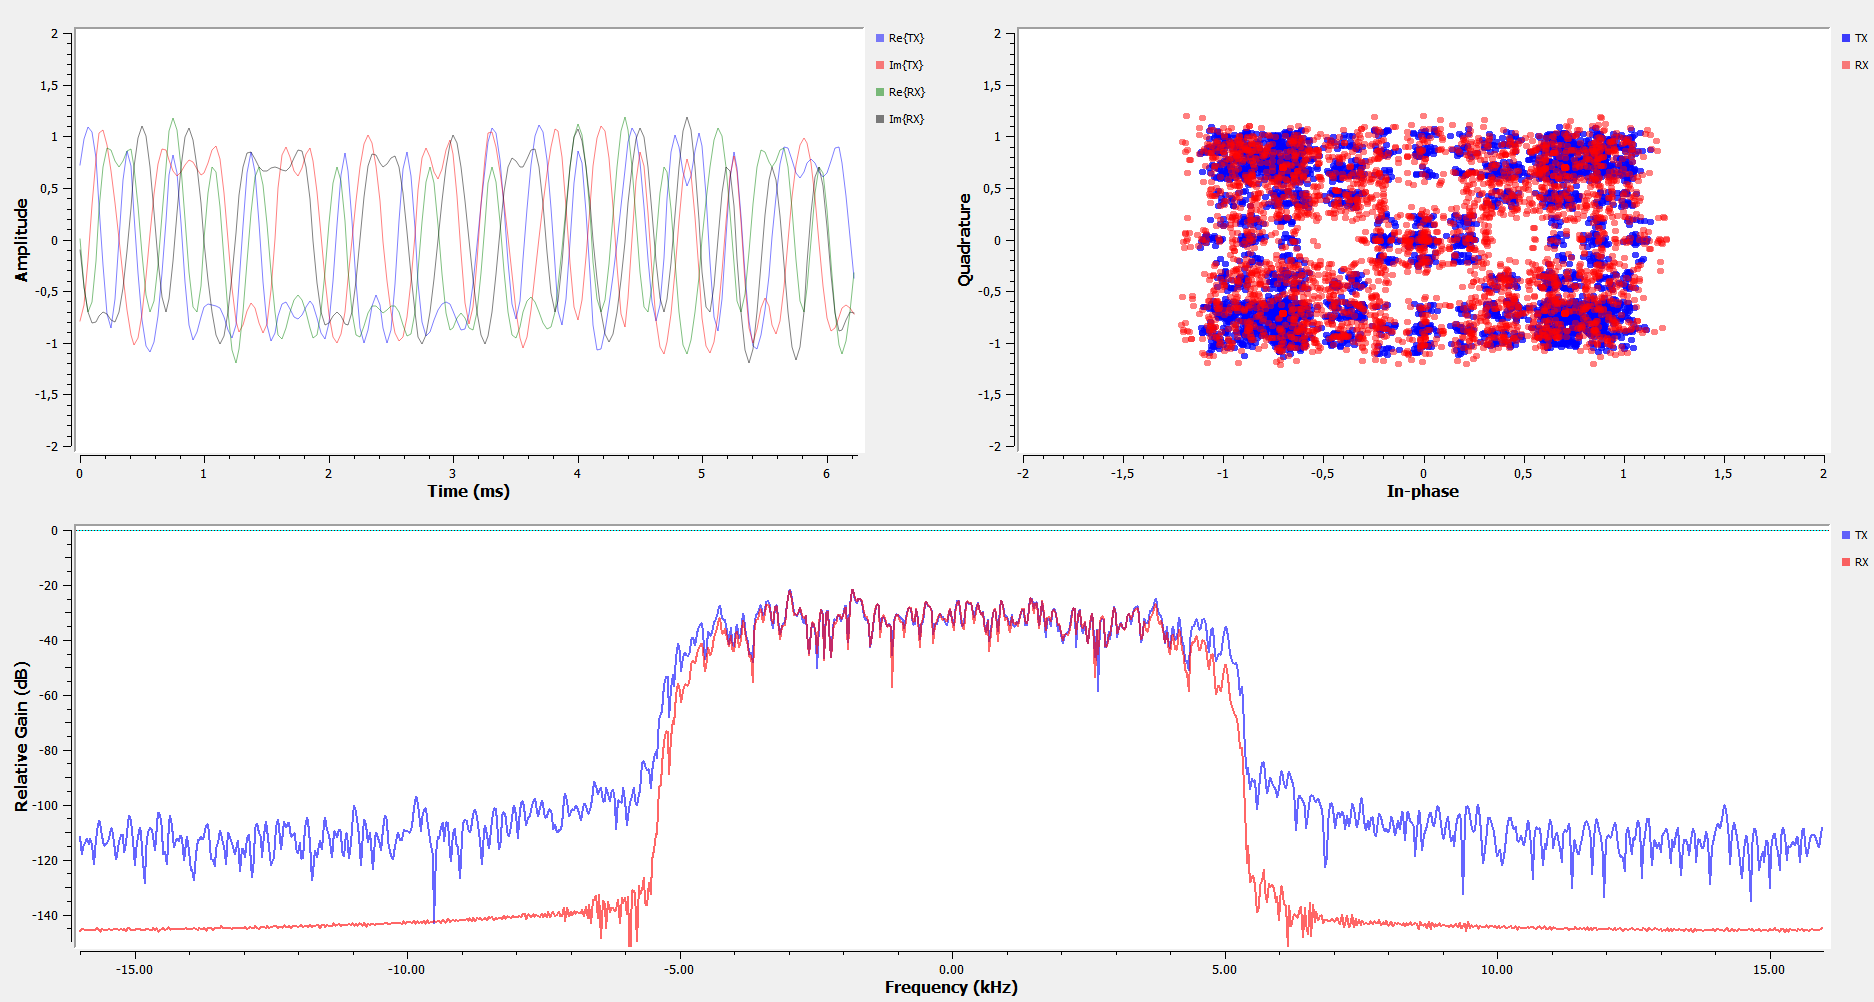
\includegraphics[width=\textwidth]{ex_1_2.png}
                \caption{График \texttt{QPSK}}
                \label{fig:ex_1_2}
            \end{figure}
            
    \newpage
        \section{Часть №2: Добавление канала передачи}
           Во второй части лабораторной работы будут рассмотрены эффекты канала, то, как сигнал искажается между передачей и видимостью в приемнике. Для начала будет использоваться самый базовый блок \texttt{Channel Model} в \texttt{GNU Radio}. Этот блок позволяет смоделировать несколько основных проблем, с которыми далее приходится иметь дело. Первая проблема с приемниками - возникающий аддитивным белый гауссовый шум (AWGN). Устанавливается мощность шума, регулируя значение шумового напряжения модели канала. Здесь указывается напряжение вместо мощности, потому что необходимо узнать ширину полосы сигнала, чтобы правильно рассчитать мощность. Другой существенной проблемой является нахождение идеальной точки выборки. Была увеличена частота дискретизации сигнала в передатчике, и он был сформирован, но при его получении необходимо произвести выборку сигнала в исходной точке выборки, чтобы максимизировать мощность сигнала и минимизировать межсимвольные помехи. Как и в имитации этапа 1 после добавления второго фильтра \texttt{RRC}, можно видеть, что среди четырех выборок на символ одна из них находится в идеальной точке выборки +1, -1 или 0. Но опять же, две радиостанции работает на разных скоростях, поэтому идеальная точка отбора проб неизвестна. 
           
           Второй этап моделирования позволяет провести эксперименты над эффектами аддитивного шума, смещения частоты и смещения синхронизации. Было добавлено немного шума (0.2), некоторое смещение частоты 0.025) и некоторое временное смещение (1.0005), чтобы увидеть результирующий сигнал с начального его положения.
           
           \begin{figure}[H]
                \centering
                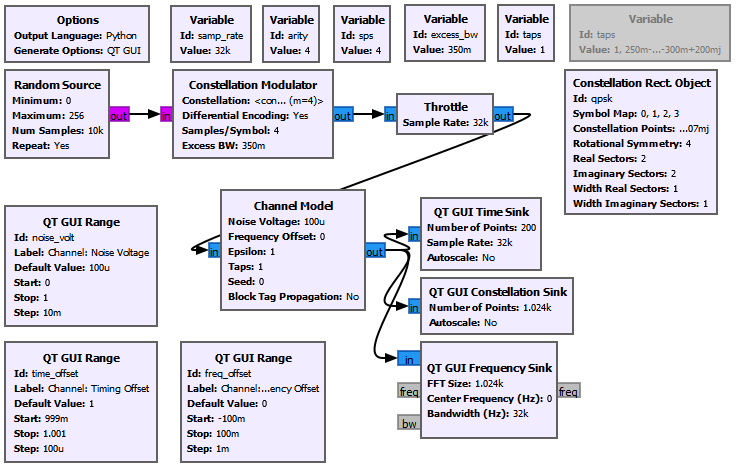
\includegraphics[width=\textwidth]{ex_2_1.png}
                \caption{Добавление канала передачи}
                \label{fig:ex_2_1}
            \end{figure}
           
           На графиках результата второго этапа изображенв исходный сигнал с наложенными на него искажениями канала. Из исходного созведия мы получили облако точек, из которого нужно будет в дальшнейшем выделить наш сигнал.
           
           \begin{figure}[H]
                \centering
                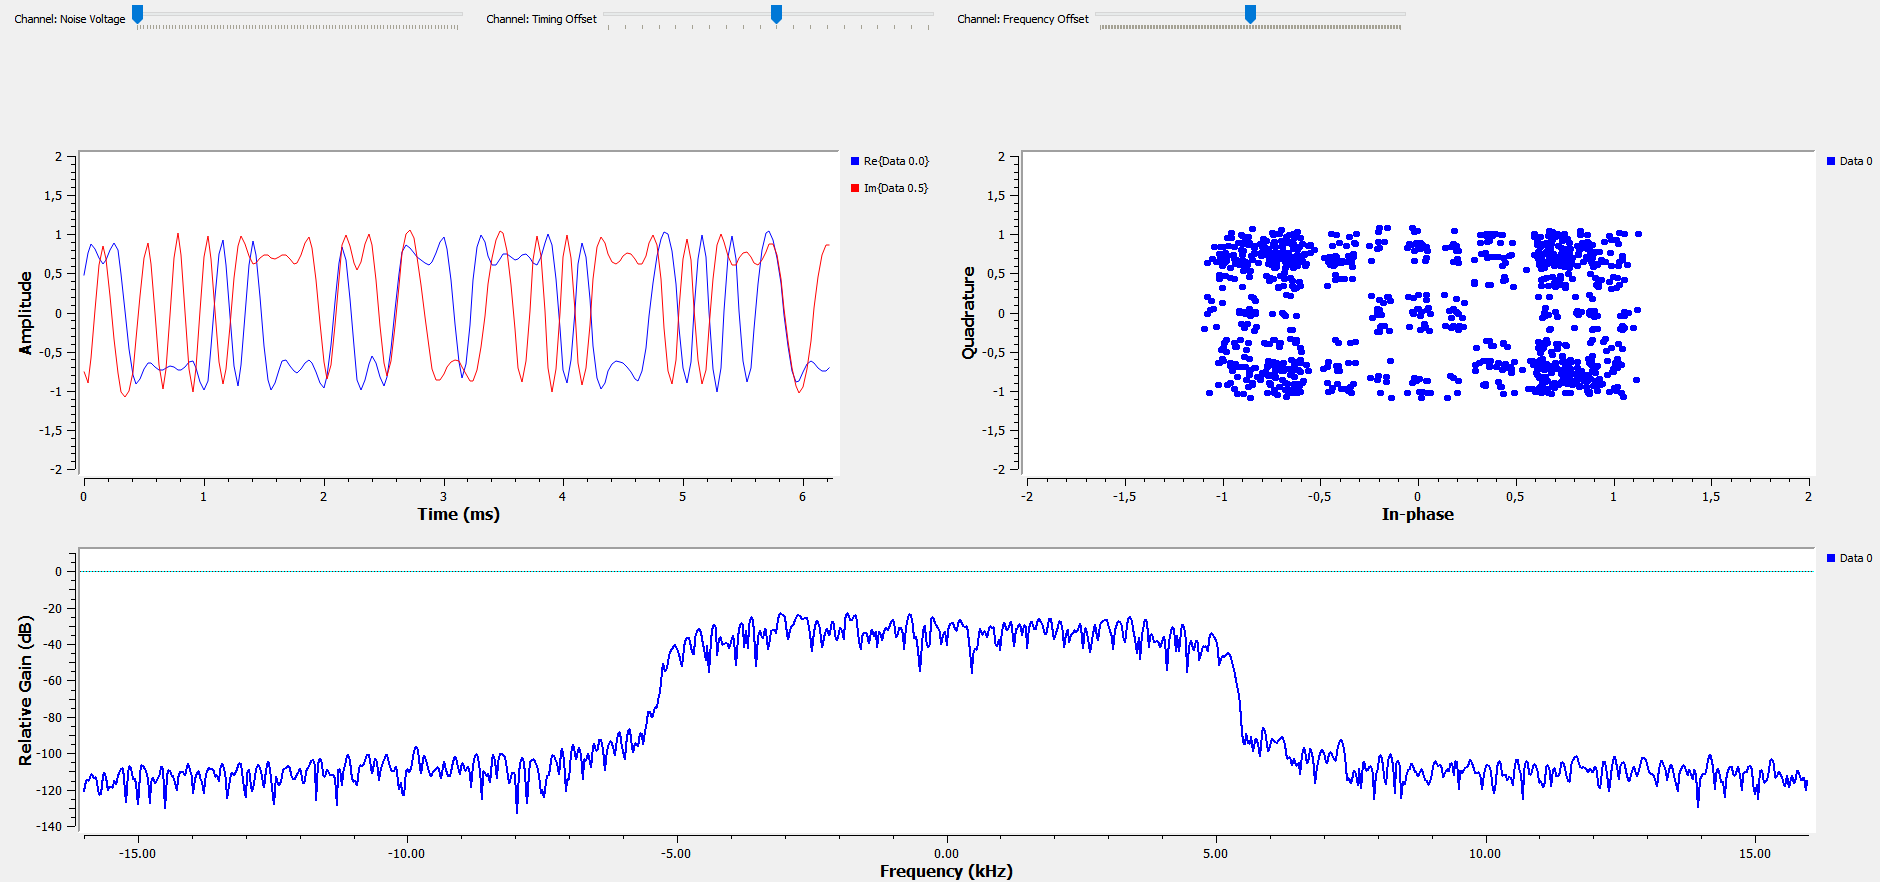
\includegraphics[width=\textwidth]{ex_2_2.png}
                \caption{Первый график результата}
                \label{fig:ex_2_2}
            \end{figure}
           
           \begin{figure}[H]
                \centering
                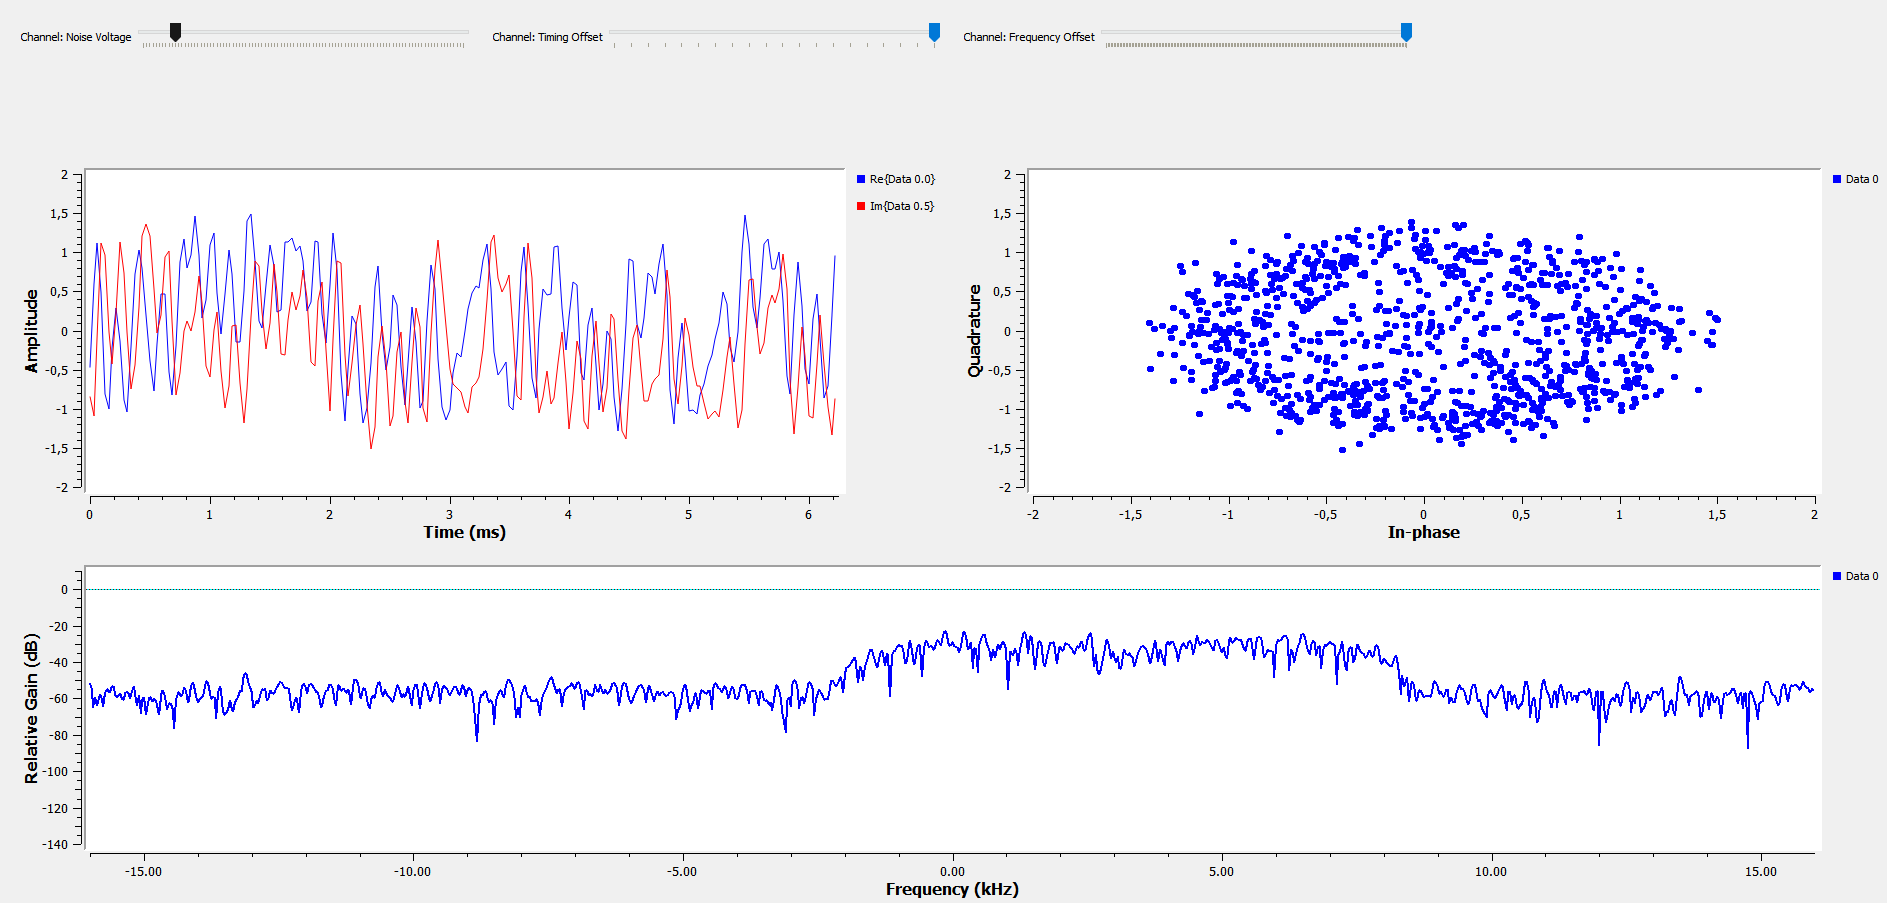
\includegraphics[width=\textwidth]{ex_2_3.png}
                \caption{Второй график результата}
                \label{fig:ex_2_3}
            \end{figure}
           
    \newpage
        \section{Часть №3: Восстановление времени}
           В третьей части лабораторной работы будет пройден процесс восстановления. Будет использоваться алгоритм \texttt{polyphase clock recovery} . Первым шагом будет восстановление времени. Задачей является найти лучшее время для выборки входящих сигналов, что позволит максимизировать отношение сигнал / шум (\texttt{SNR}) каждого образца, а также уменьшить влияние межсимвольных помех (\texttt{ISI}).
           
           Можно проилюстрировать проблему \texttt{ISI}, используя пример \texttt{flowgraph \\symbolsampling}. Первый этап фильтрации изменяет частоту выборки до значения ’ \texttt{sps} ’ на элемент и использует \texttt{ISI} \texttt{root raised cosine} фильтр. За этим следует другой \texttt{root raised cosine} фильтр, который не изменяет скорость. Второй фильтр \texttt{RRC} здесь преобразует сигналы от использования не\texttt{-Nyquist} \texttt{RRC}-фильтра в \texttt{Nyquist raised cosine (RC)} фильтр. Можно наблюдать как восстановление синхронизации применяет согласованный фильтр для удовлетворения критерию \texttt{Nyquist ISI}.
            
            \begin{figure}[H]
                \centering
                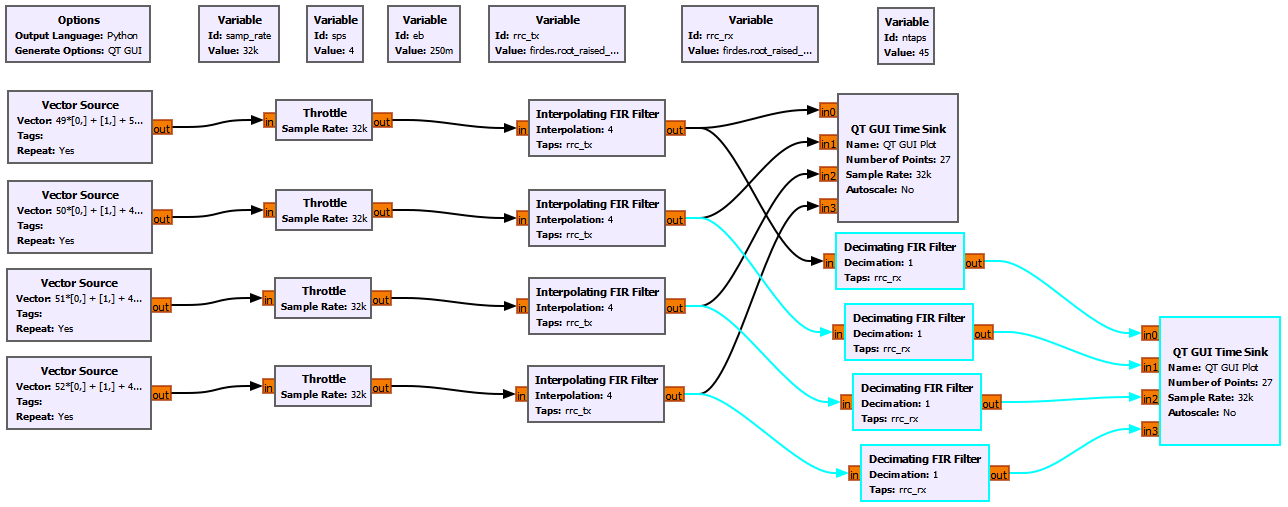
\includegraphics[width=\textwidth]{ex_3_1.png}
                \caption{Схема без рассинхронизации}
                \label{fig:ex_3_1}
            \end{figure}
            
            \begin{figure}[H]
                \centering
                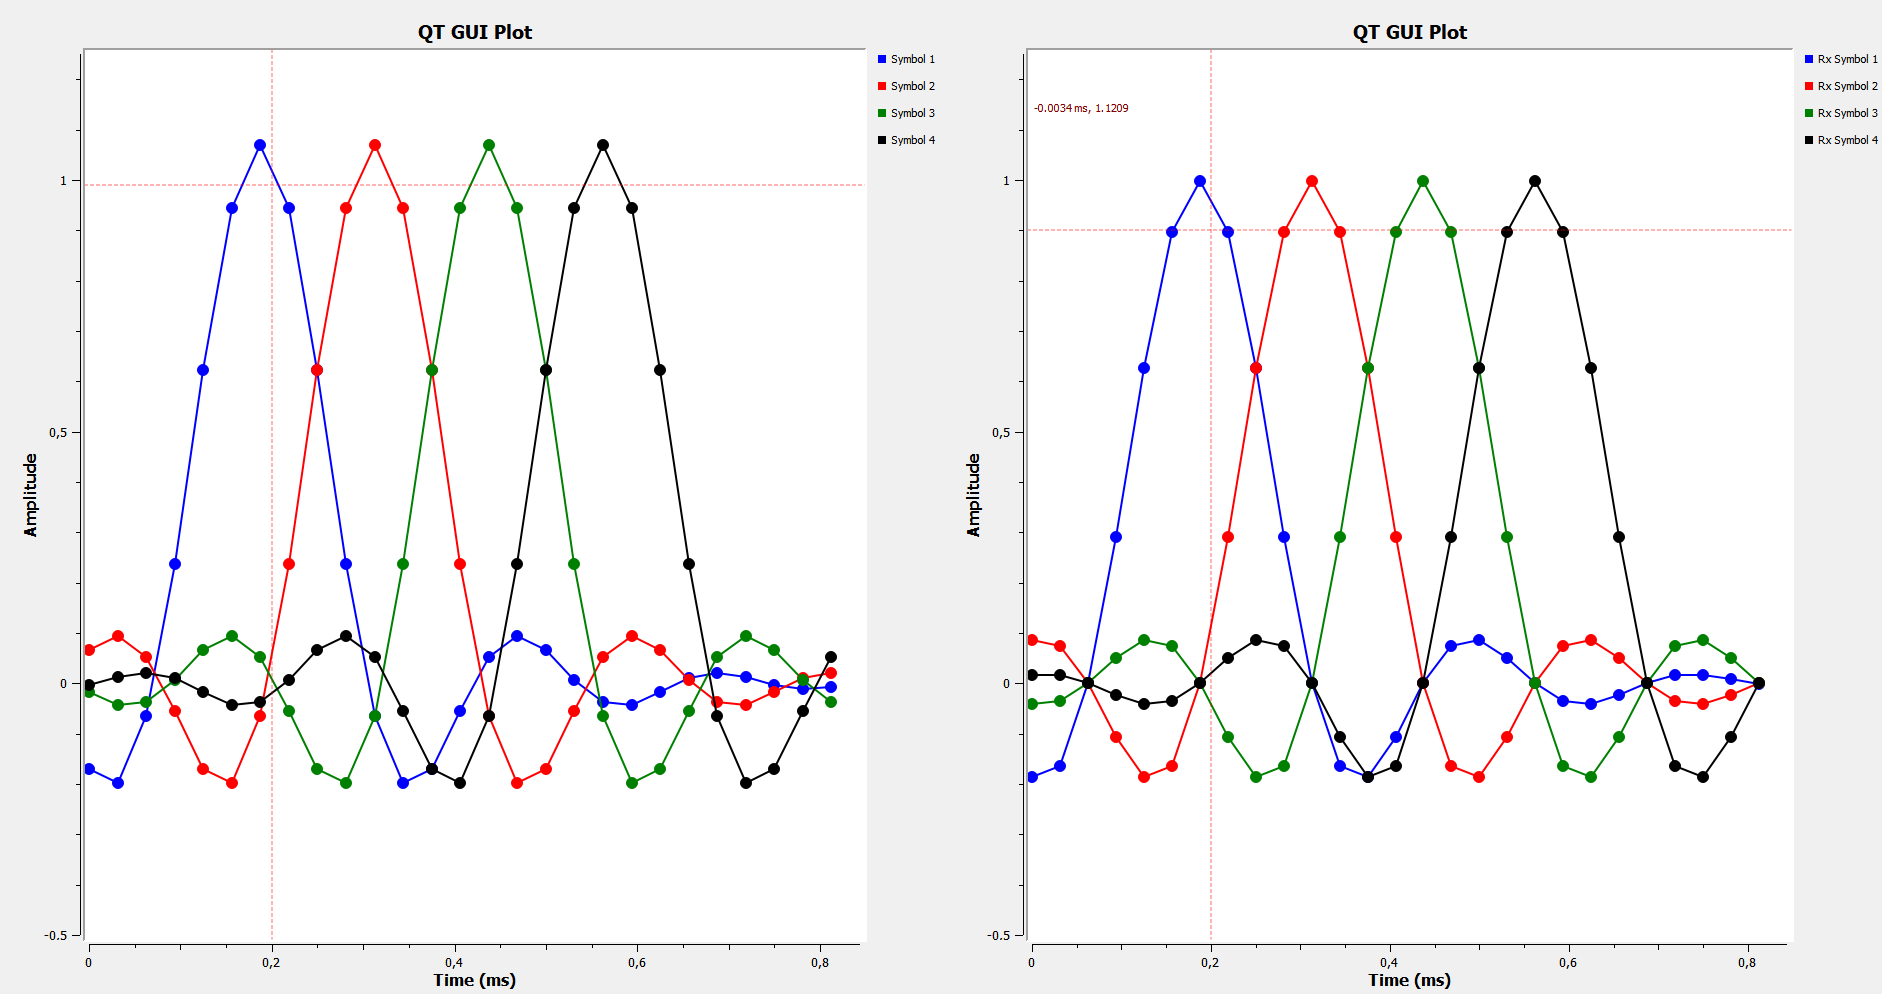
\includegraphics[width=\textwidth]{ex_3_2.png}
                \caption{Передача четырех символов без рассинхронизации}
                \label{fig:ex_3_2}
            \end{figure}
            
            \begin{figure}[H]
                \centering
                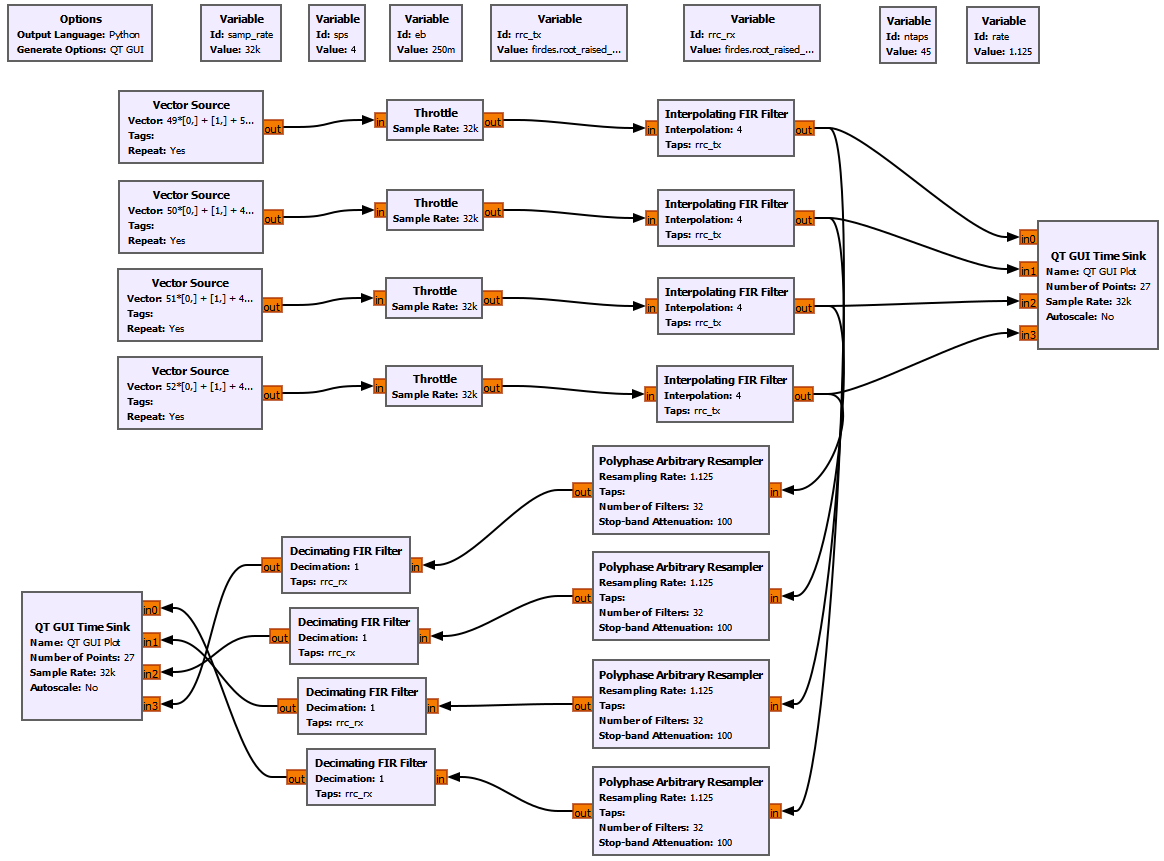
\includegraphics[width=\textwidth]{ex_3_3.png}
                \caption{Схема со рассинхронизацией}
                \label{fig:ex_3_3}
            \end{figure}
            
            \begin{figure}[H]
                \centering
                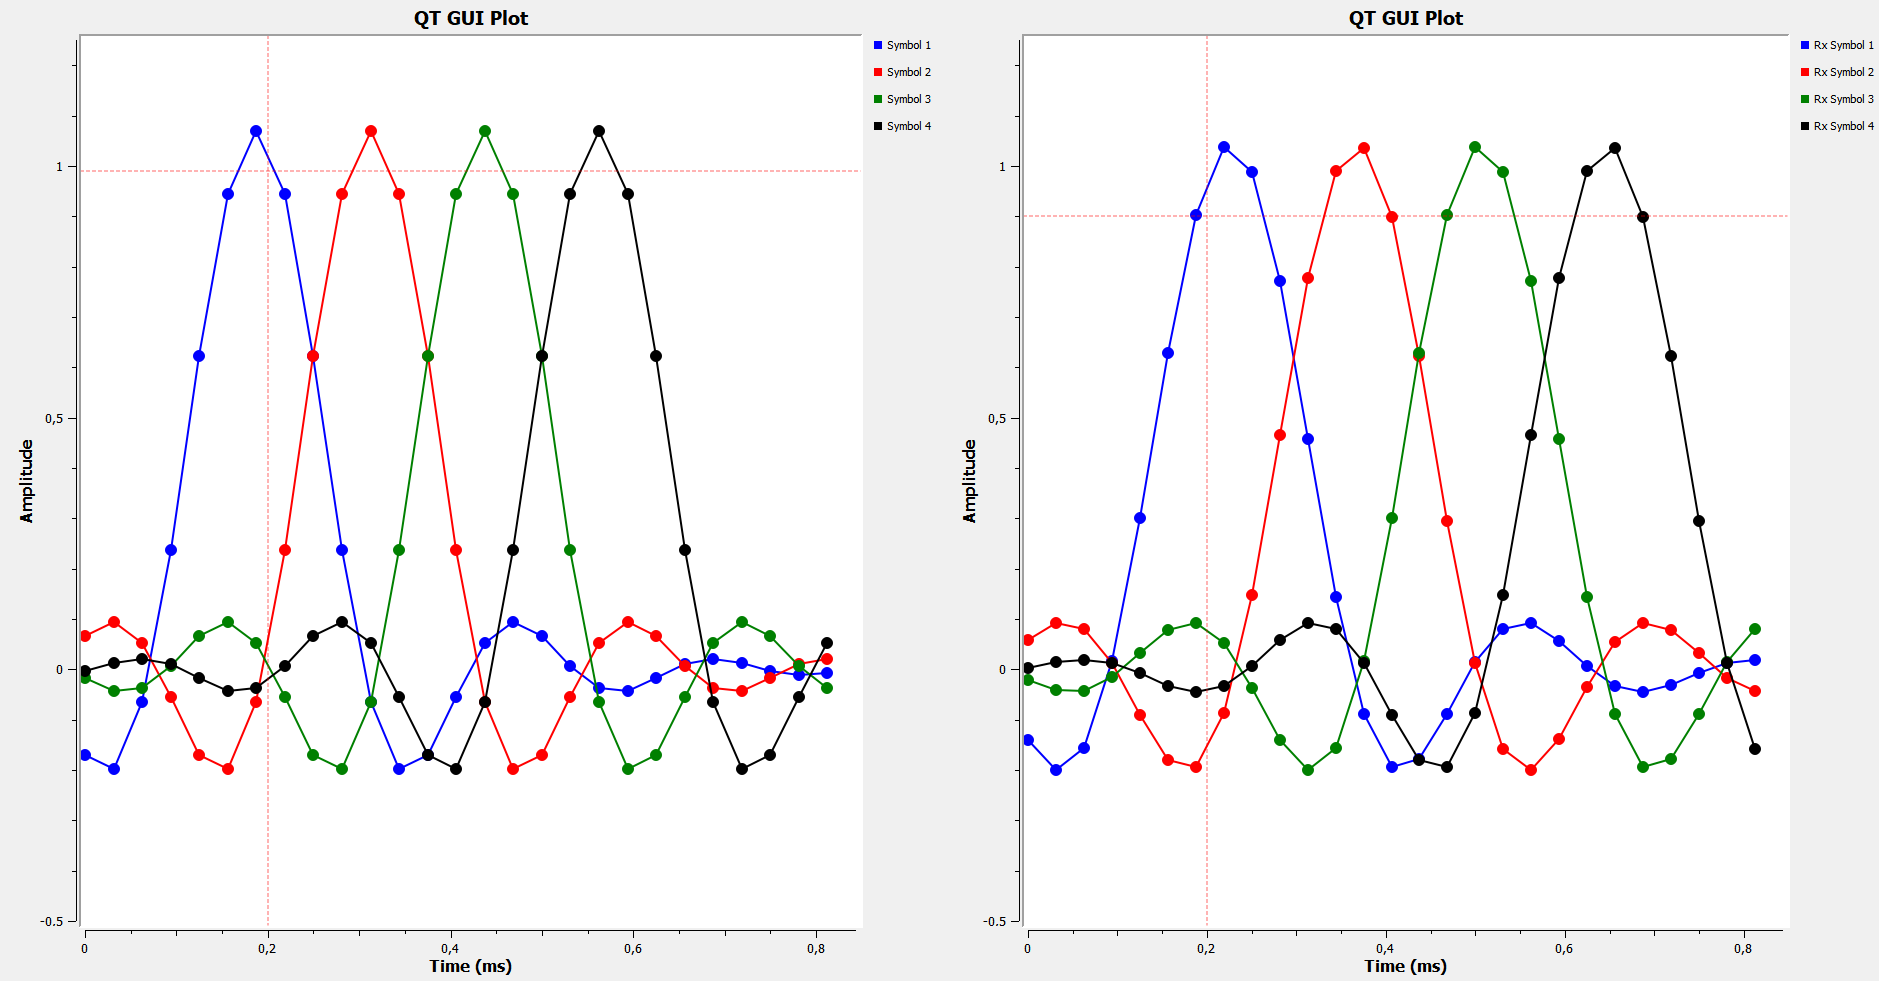
\includegraphics[width=\textwidth]{ex_3_4.png}
                \caption{Передача четырех символов с рассинхронизацией}
                \label{fig:ex_3_4}
            \end{figure}
            
            Для восстановления времени на приемнике будет использоваться метод восстановления тактового сигнала многофазного фильтра. Этот блок выполняет восстановление времени и избавляет от проблемы \texttt{ISI}. Он работает путем вычисления первого дифференциала входящего сигнала, который будет связан с его тактовым смещением. Выборка, которую хочется видеть, находится в 0.25 мс. Разностный фильтр ([-1, 0, 1]) генерирует дифференциал символа, и, как показано на следующем рисунке, выход этого фильтра в правильной точке выборки равен 0. Оптимальная точка выборки считается найденной тогда, когда выход дифференциального фильтра равен 0.
            
            \begin{figure}[H]
                \centering
                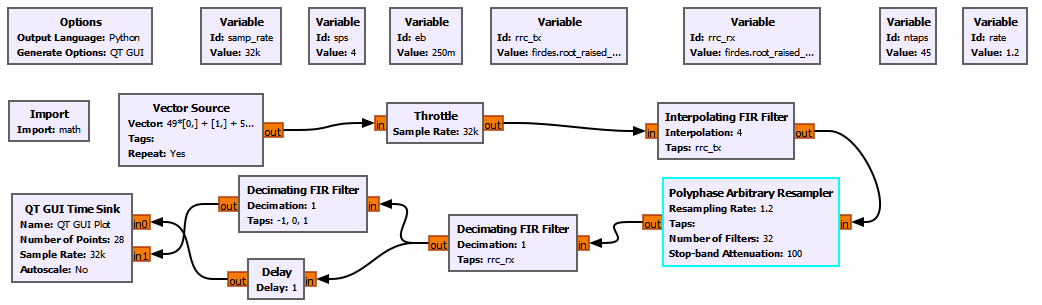
\includegraphics[width=\textwidth]{ex_3_5.png}
                \caption{Схема}
                \label{fig:ex_3_5}
            \end{figure}
            
            \begin{figure}[H]
                \centering
                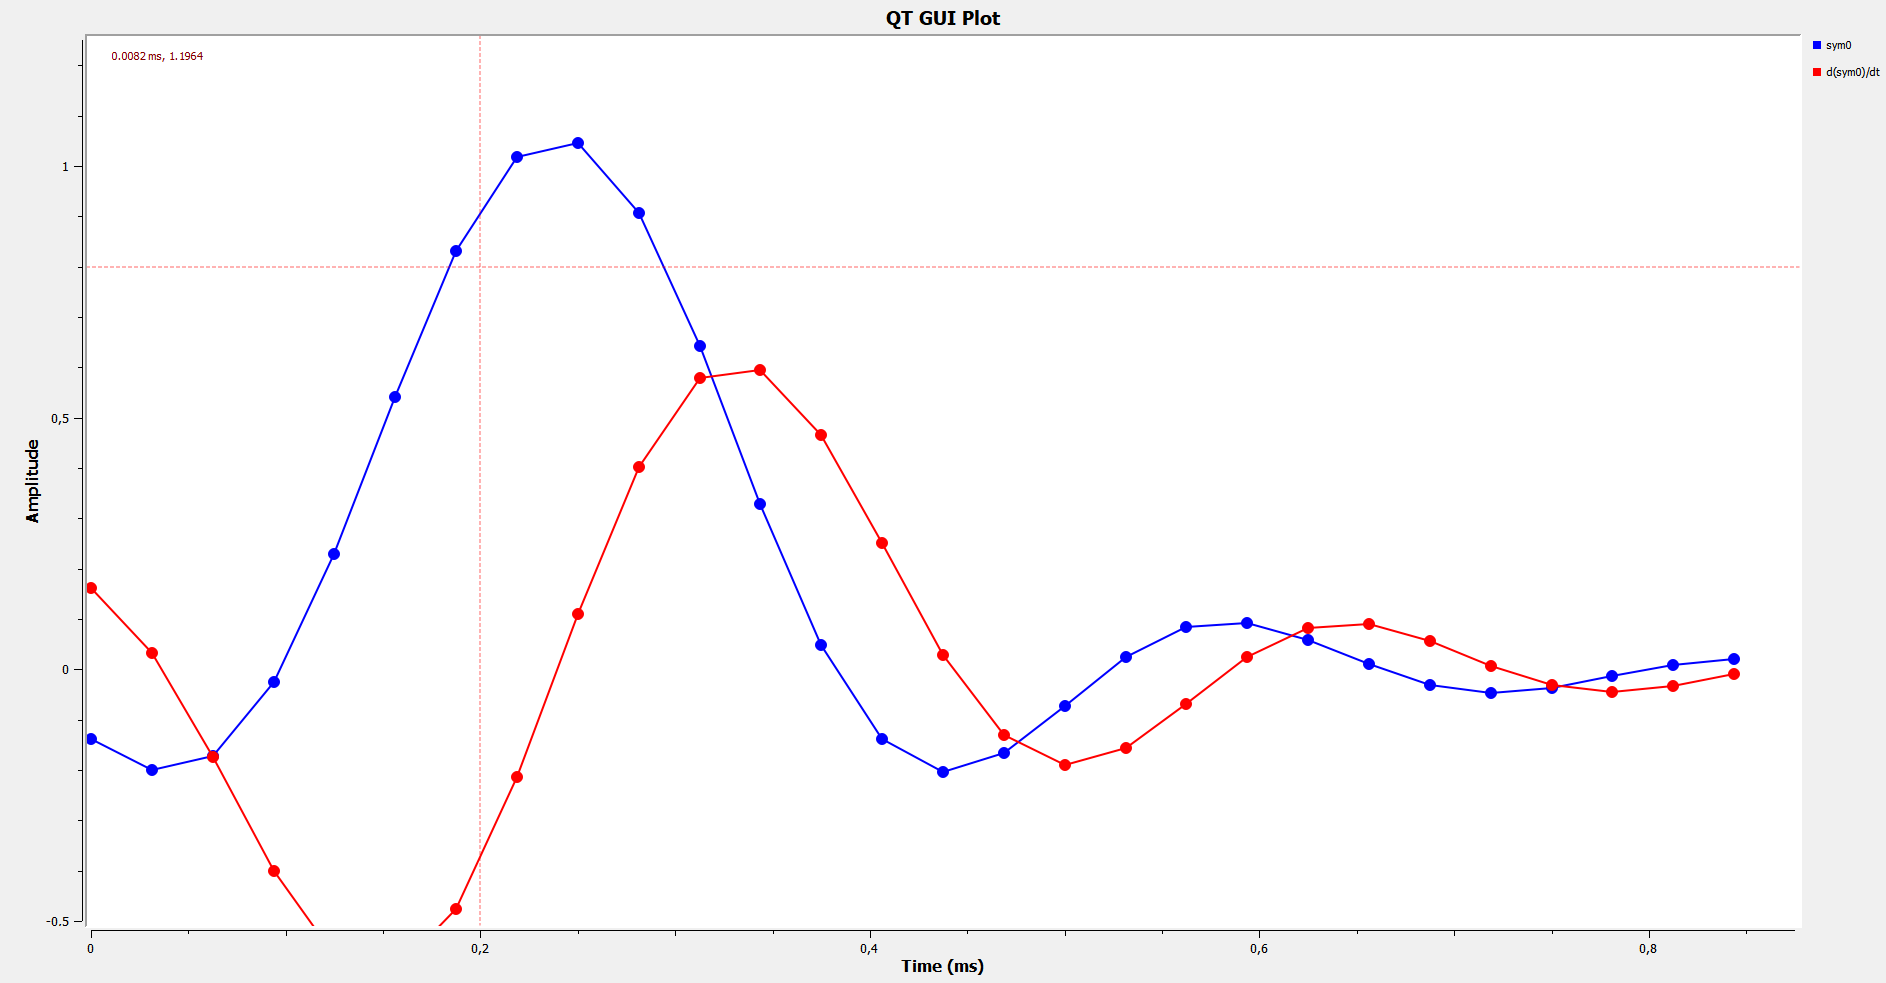
\includegraphics[width=\textwidth]{ex_3_6.png}
                \caption{Синхронизация}
                \label{fig:ex_3_6}
            \end{figure}
            
            Было рассмотренно моделирование, которое использует 5 фильтров(т.е 5 различных фаз). В данном случае используется \texttt{fractional resampler}, так как он позволяет легко произвести сдвиг фазы (между 0 и 1), и он также изменяет задержку фильтра сигналов, что необходимо скореектировать с помощью блоков задержки.
            
            Можно видеть, что сигнал d(sym0)/dt + phi3 имеет точку отсчета ровно в 0. Это говорит о том, что идеальная точка отсчета происходит при этом смещении фазы. Поэтому, если взять фильтр \texttt{RRC} этого приемника и отрегулировать его фазу по phi3, то мы можем исправить несоответствие времени и выбрать идеальную точку выборки.
            
            Была компенсирована частота дискретизации некоторым известным коэффициентом 1.2 и оказалось, что можно использовать один из пяти фильтров в качестве идеальной точки выборки. Любое смещение выборки между этими фазами все еще будет производить несвоевременную выборку с добавлением \texttt{ISI} как исследовали ранее. Поэтому вместо этого используется более 5 фильтров в данном алгоритме восстановления.
            
            \begin{figure}[H]
                \centering
                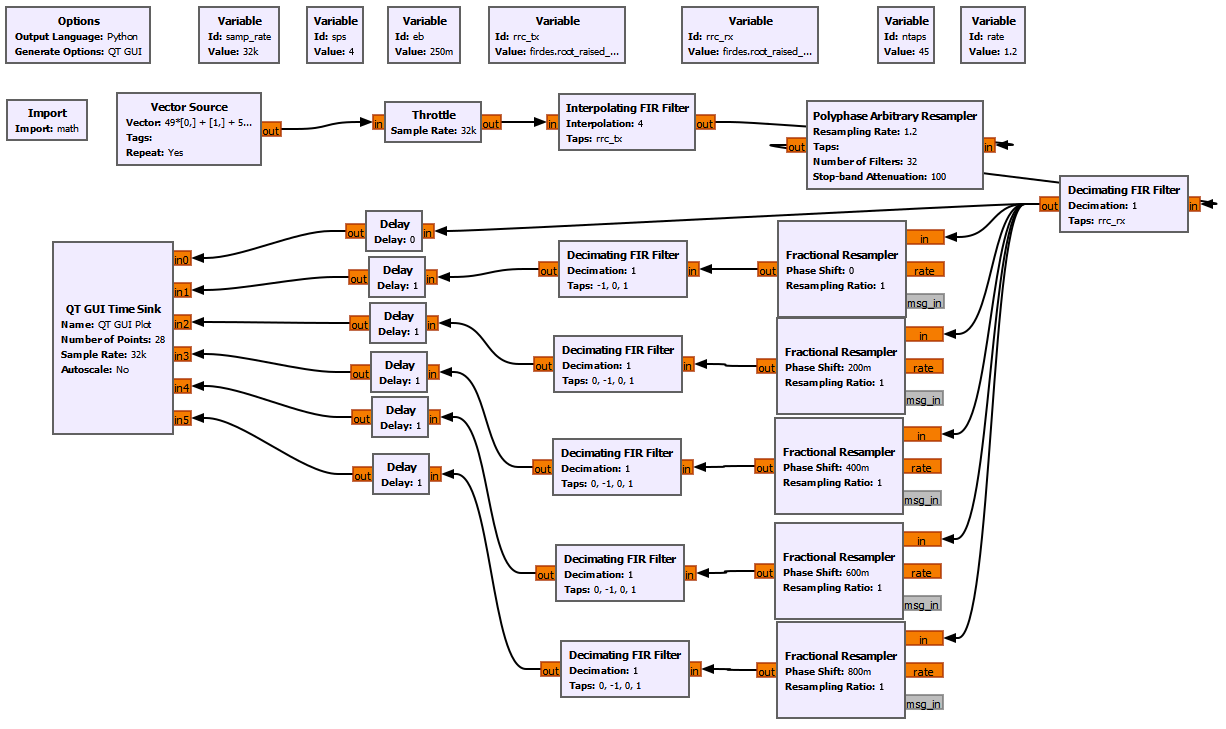
\includegraphics[width=\textwidth]{ex_3_7.png}
                \caption{Схема со синхронизацией}
                \label{fig:ex_3_7}
            \end{figure}
            
            \begin{figure}[H]
                \centering
                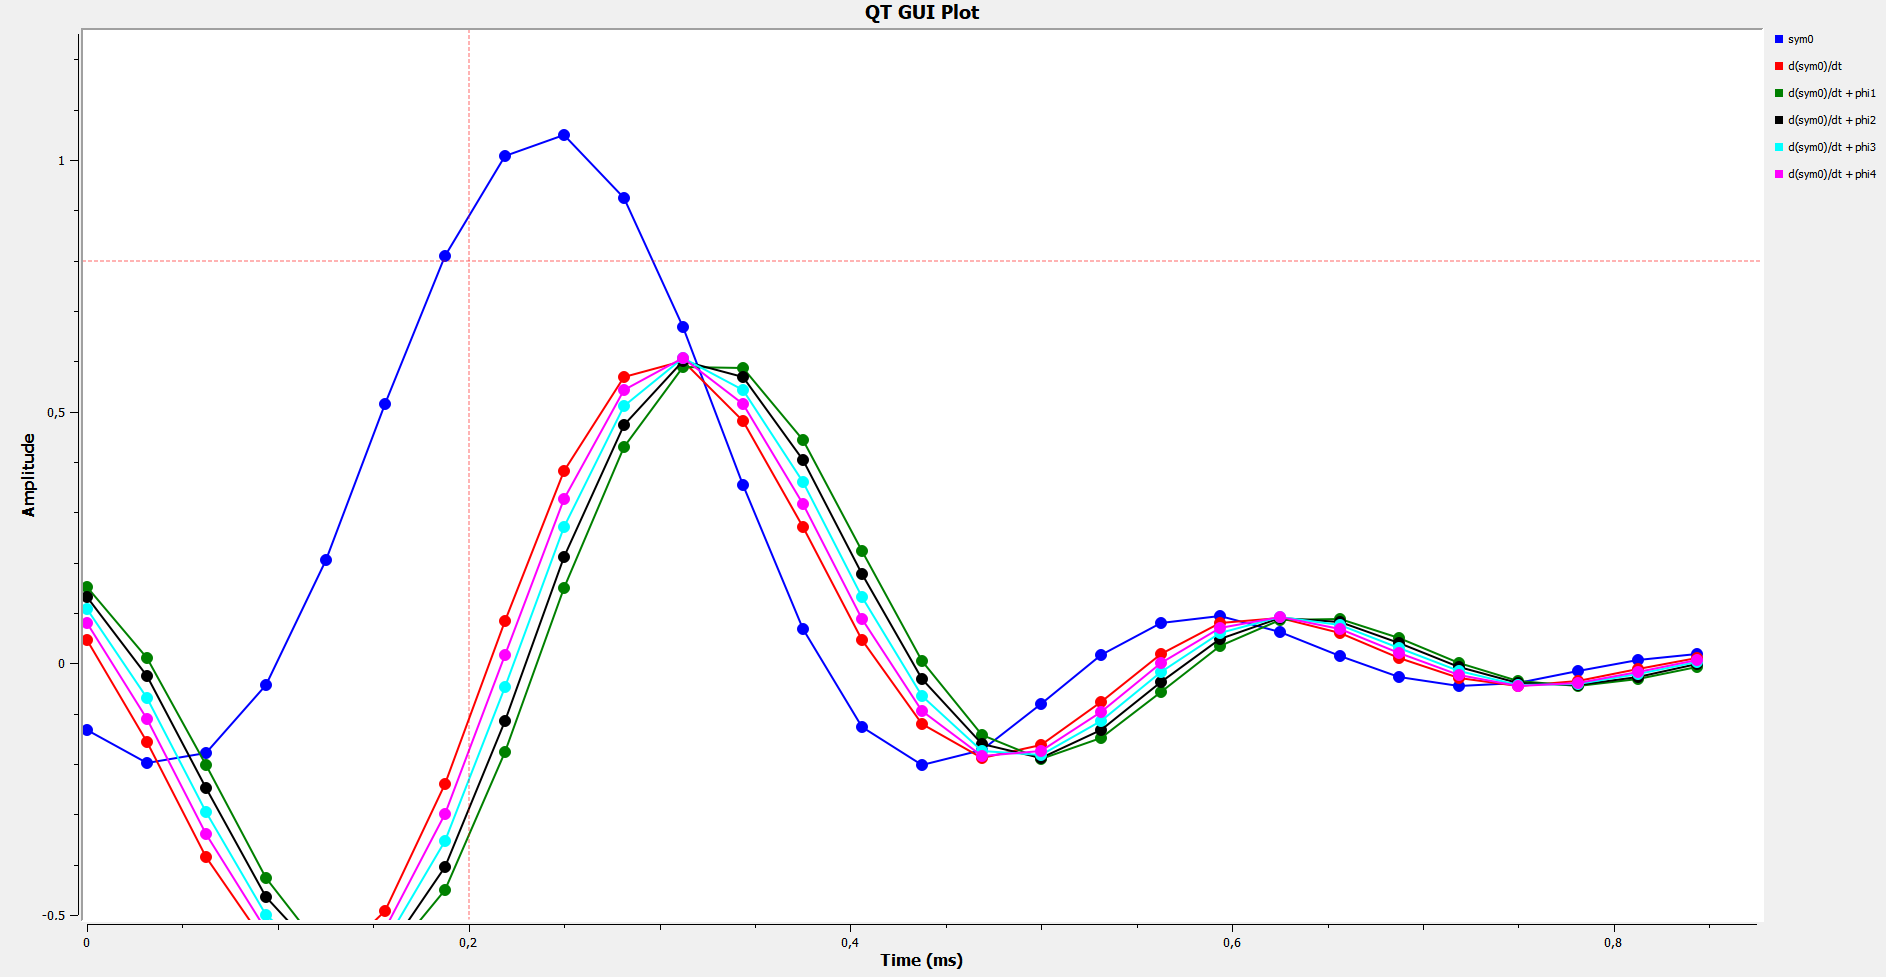
\includegraphics[width=\textwidth]{ex_3_8.png}
                \caption{Расширенный экран синхронизации}
                \label{fig:ex_3_8}
            \end{figure}
            
    \newpage
        \section{Часть №4: Восстановление синхронизации}
            В четвертом пункте лабораторной работы будет использоваться результат упомянутых выше рассуждений.
            
            Данный граф \texttt{mpskstage3.gcr} принимает выходной сигнал модели канала и пропускает его через наш многофазный блок синхронизации часов. Этот блок настроен с 32 фильтрами и пропускной способностью петли 2pi/100, принимает значение для ожидаемых выборок на символ. Внутренне, блок будет адаптироваться вокруг этого значения на основе скорости входящего сигнала. Можно наблюдать сближение созвездия.
            
            \begin{figure}[H]
                \centering
                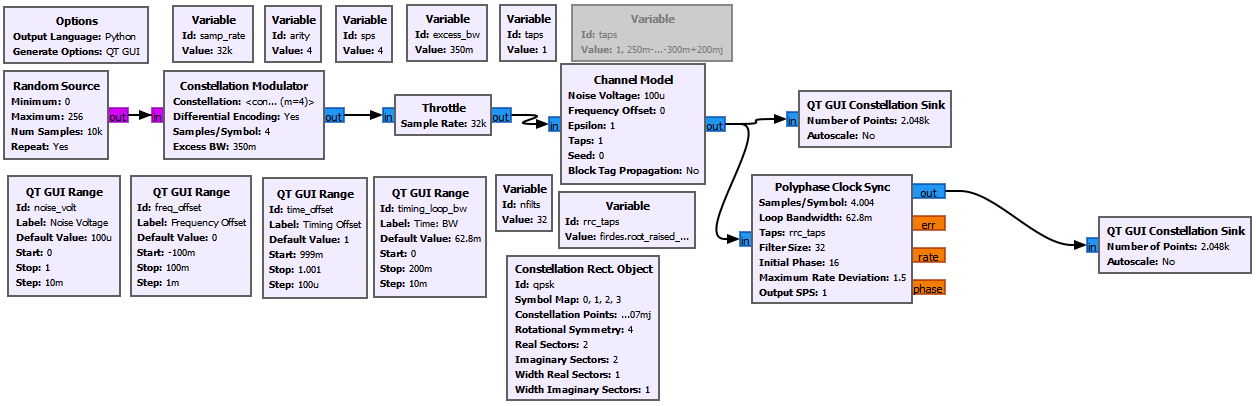
\includegraphics[width=\textwidth]{ex_4_1.png}
                \caption{Схема 3 шага}
                \label{fig:ex_4_1}
            \end{figure}
            
            При запуске этого сценария отображается созвездие: слева как полученный сигнал до восстановления синхронизации и справа после восстановления синхронизации. Изображение все еще немного зашумленно в результате \texttt{ISI} после 32 фильтров.
            
            Когда происходит смещение частоты, можно видеть, что созвездие становится кругом. Однако блок все еще не позволяет исправить смещение частоты. Аналогичным образом, можно изменить среду многолучевого моделирования, изменив переменную taps. Добавление \texttt{multipath} покажет, что блок восстановления времени устойчив к \texttt{multipath}, но не будет исправлять его, поэтому снова нужно прибегнуть к дополнительным методам решения проблемы.
            
            \begin{figure}[H]
                \centering
                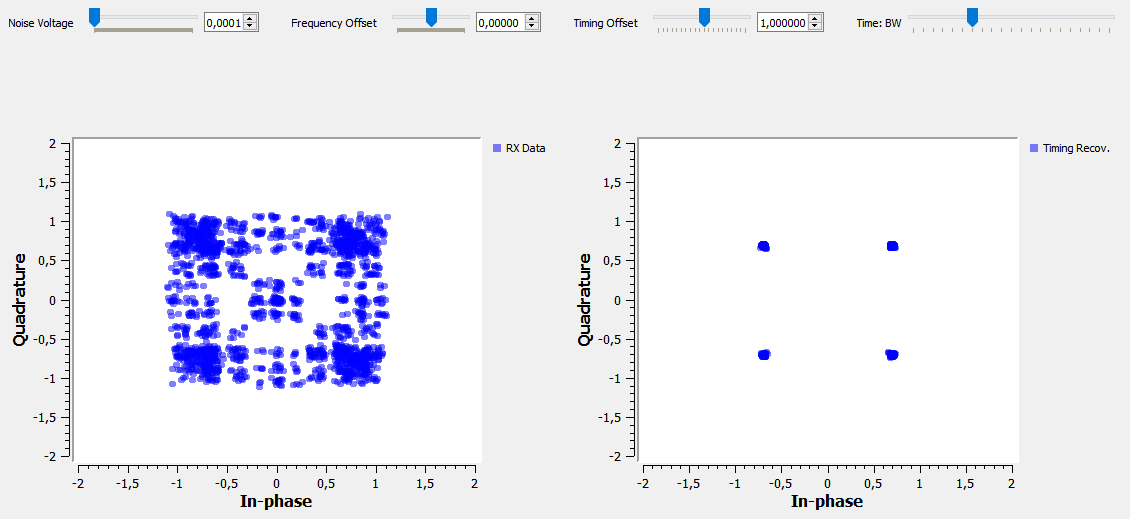
\includegraphics[width=\textwidth]{ex_4_2.png}
                \caption{Первая схема синхронизации}
                \label{fig:ex_4_2}
            \end{figure}
            
            \begin{figure}[H]
                \centering
                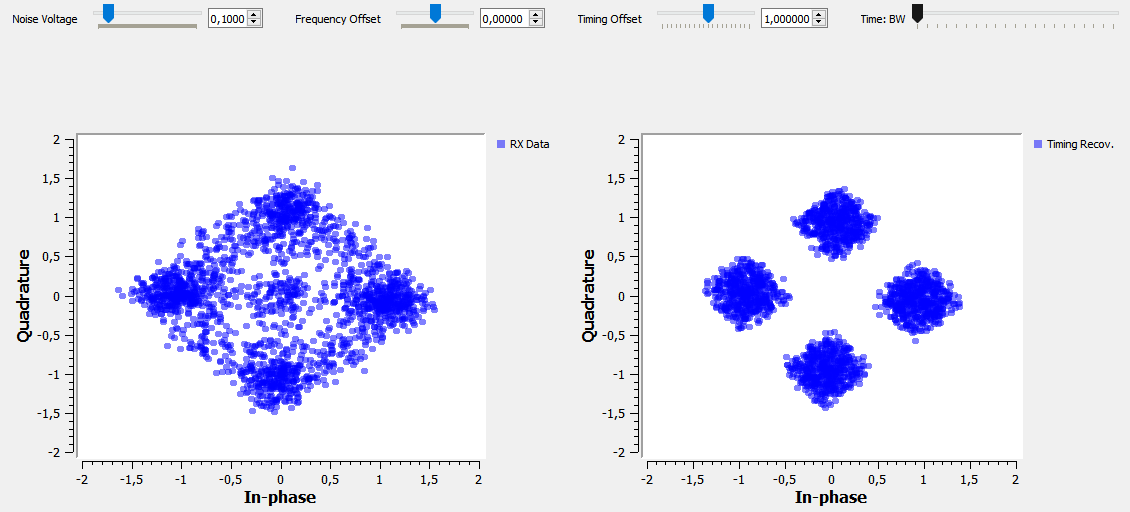
\includegraphics[width=\textwidth]{ex_4_3.png}
                \caption{Вторая схема синхронизации}
                \label{fig:ex_4_3}
            \end{figure}
            
    \newpage
        \section{Часть №5: Многолучевое распространение}
            В пятом пункте лабораторной работы будем рассмотривать многолучевое распространение. \\\texttt{Multipath} является результатом того факта, что в большинстве коммуникационных сред нет единого пути для передачи сигнала от передатчика к приемнику. Каждый раз, когда есть объект, отражающий сигнал, между двумя узлами может быть установлен новый путь. Каждый из этих отражающих путей будет отображаться на приемнике в разное время в зависимости от длины пути. Суммирование их вместе у приемника вызывает искажения. Если разница во времени между отражениями достаточно мала относительно ширины символа, то искажение может быть внутри символа – внутрисимвольная интерференция. Когда отражения будут длиннее времени символа, отражение от одного символа повлияет на следующие сигналы - еще одна причина для интерференции между символами. Нужно исправить это поведение с помощью механизма, очень похожего на стереоэквалайзер (уравнитель). С помощью стереоэквалайзера можно изменить усиление определенных частот, чтобы либо подавить, либо усилить эти сигналы-бас и высокие частоты являются общими.
            
            \texttt{Multipathsim.grc} просто устанавливает модель канала, чтобы обеспечить канал с пятью кнопками эквалайзера, четыре из которых можем изменить. На рисунке ниже многолучевой канал создает некоторое искажение в сигнале. Задача эквалайзера - инвертировать этот канал. Необходимым является ипользование подходящего алгоритма эквалайзера и правильная настройка параметров. Одним из важных из них в данном эксперименте является количество нажатий в эквалайзере. Как можно видеть при моделировании, пять отводов дают довольно грубый контроль над частотной характеристикой. Также, чем больше отводов, тем больше времени требуется как для вычисления отводов, так и для запуска эквалайзера против сигнала.
            
            \begin{figure}[H]
                \centering
                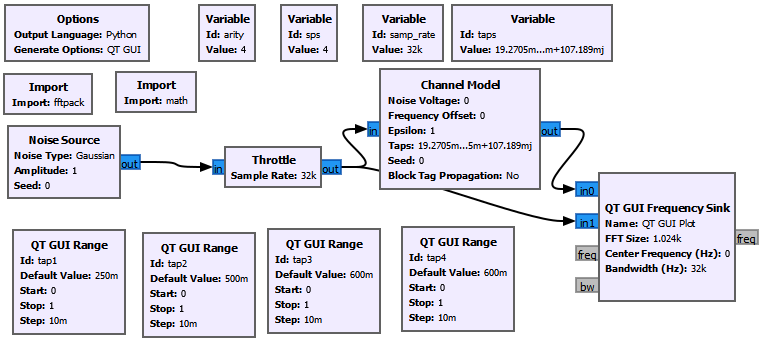
\includegraphics[width=\textwidth]{ex_5_1.png}
                \caption{Схема}
                \label{fig:ex_5_1}
            \end{figure}
            
            \begin{figure}[H]
                \centering
                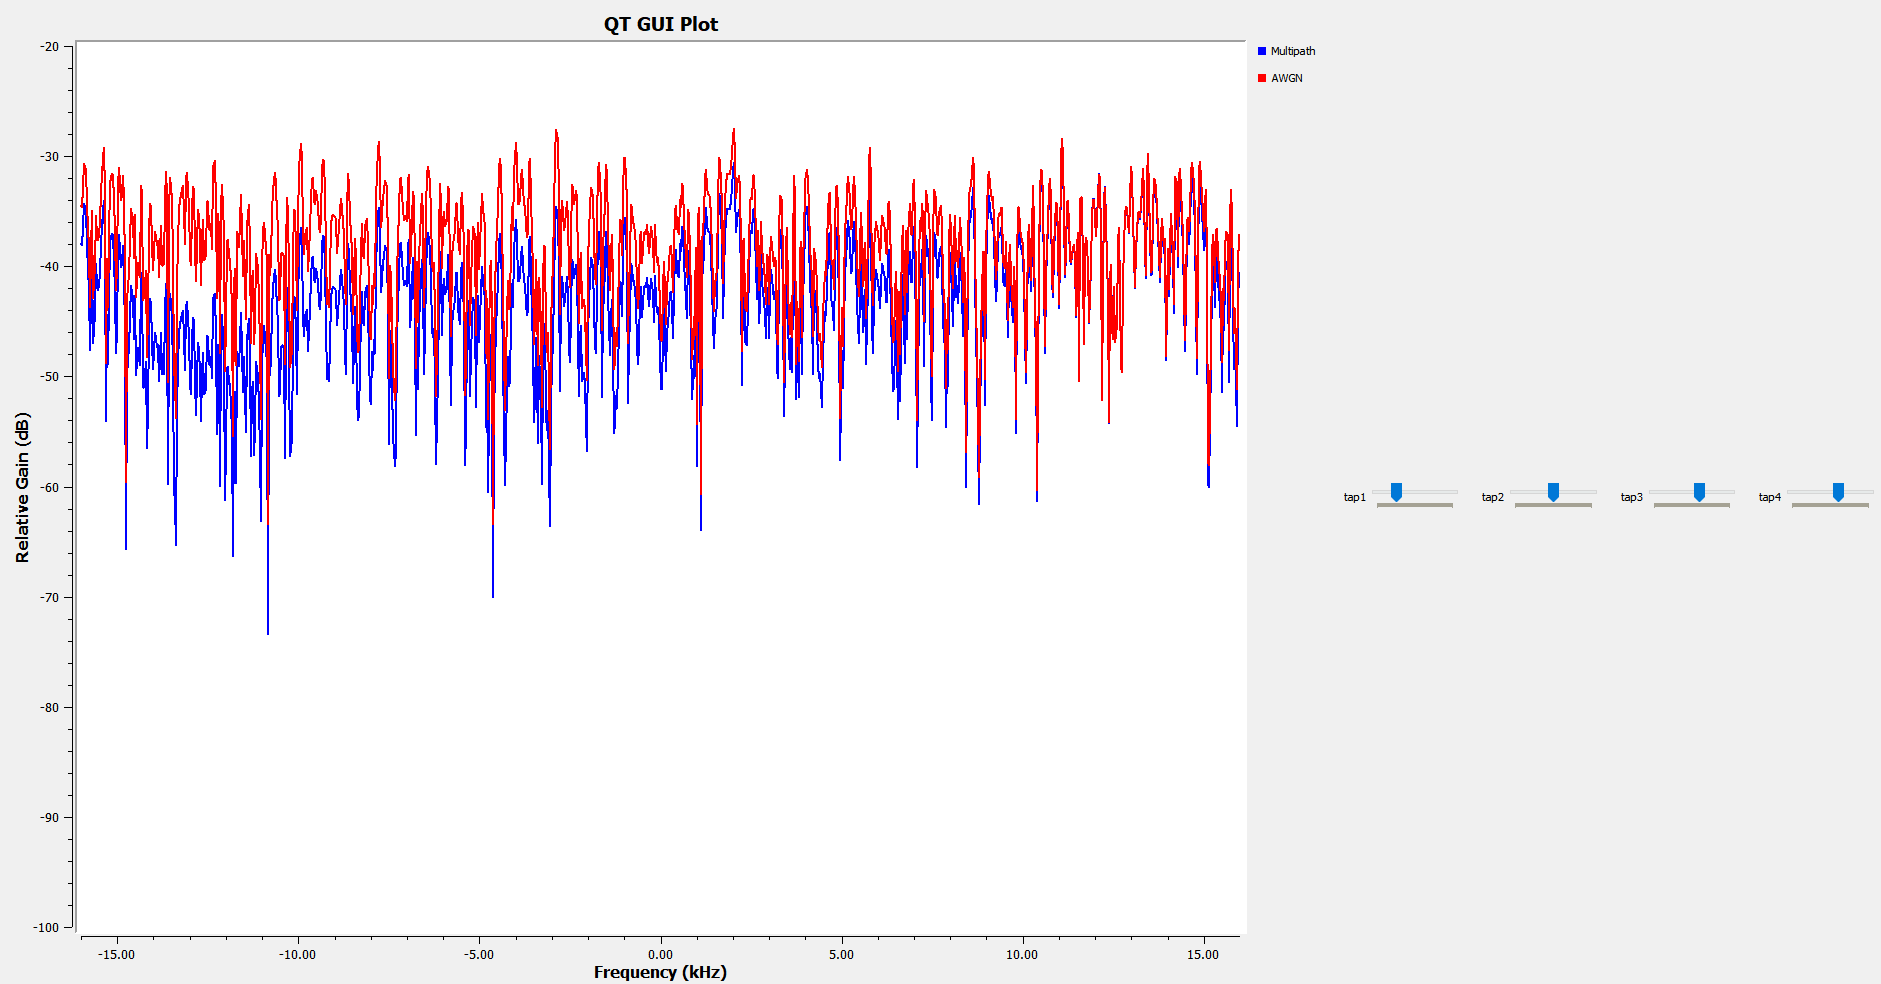
\includegraphics[width=\textwidth]{ex_5_2.png}
                \caption{График многолучевого распространения}
                \label{fig:ex_5_2}
            \end{figure}
            
    \newpage
        \section{Часть №6: Эквалайзеры}
            В шестом пункте мы будет рассматривать эквалайзеры, поставляемые GNU Radio: эквалайзер  \texttt{CMA} и эквалайзер \texttt{LMS DD}. 
            
            \normalsize{\LARGE \textbf{CMA}}
            
             \texttt{CMA}, или алгоритм постоянного модуля, является слепым эквалайзером. Он работает только на сигналах, которые имеют постоянную амплитуду или модуль. Алгоритм  \texttt{CMA} принимает количество нажатий для использования в эквалайзере, которое будет основано на некоторой комбинации. Хочется сохранить это число небольшим, чтобы уменьшить накладные расходы алгоритма, убедившись, что есть достаточно степеней свободы, чтобы исправить для канала. 
            
            В  \texttt{mpskstage4.grc}, используется алгоритм  \texttt{CMA} с 11 отводами. Было продемонстрировано, как он влияет на производительность с вычислительной и с сигнальной точки зрения.
            
            \begin{figure}[H]
                \centering
                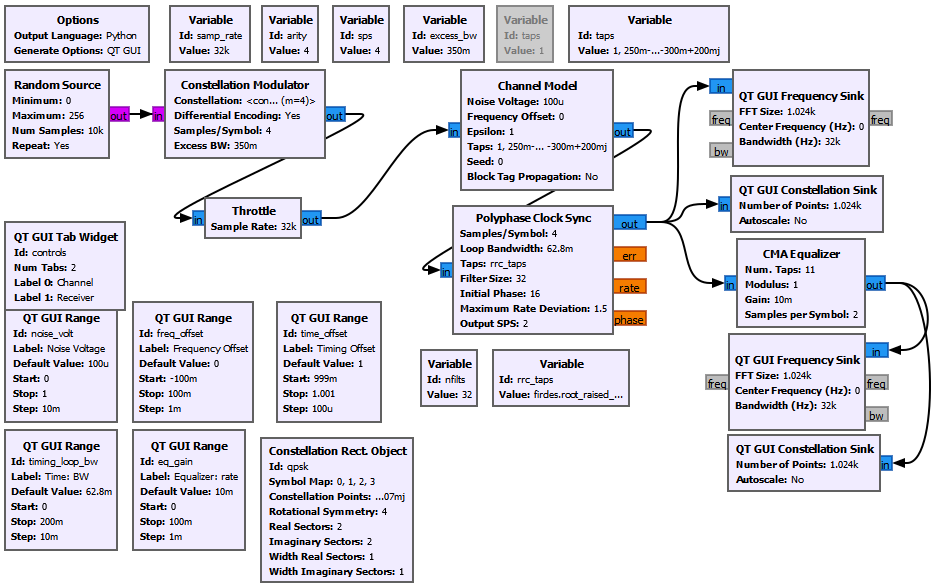
\includegraphics[width=\textwidth]{ex_6_1.png}
                \caption{Эквализация \texttt{CMA}}
                \label{fig:ex_6_1}
            \end{figure}
            
            Можно видеть, как сходится алгоритм \texttt{CMA}. Имеется блок синхронизации по времени, так и блок эквалайзера, они сходятся независимо, но одна стадия повлияет на следующую стадию. Таким образом, здесь происходит некоторое взаимодействие, когда оба фиксируются на сигнале. В конце, однако, можно видеть эффект запертого во времени многолучевого сигнала до и после эквалайзера. Перед эквалайзером имеется зашумленный, неровный сигнал. Применение эквалайзера дает возможность вновь увидеть чистый сигнал. Также можно видеть сам канал и то, как он хорошо выравнивается после эквалайзера.
            
            \begin{figure}[H]
                \centering
                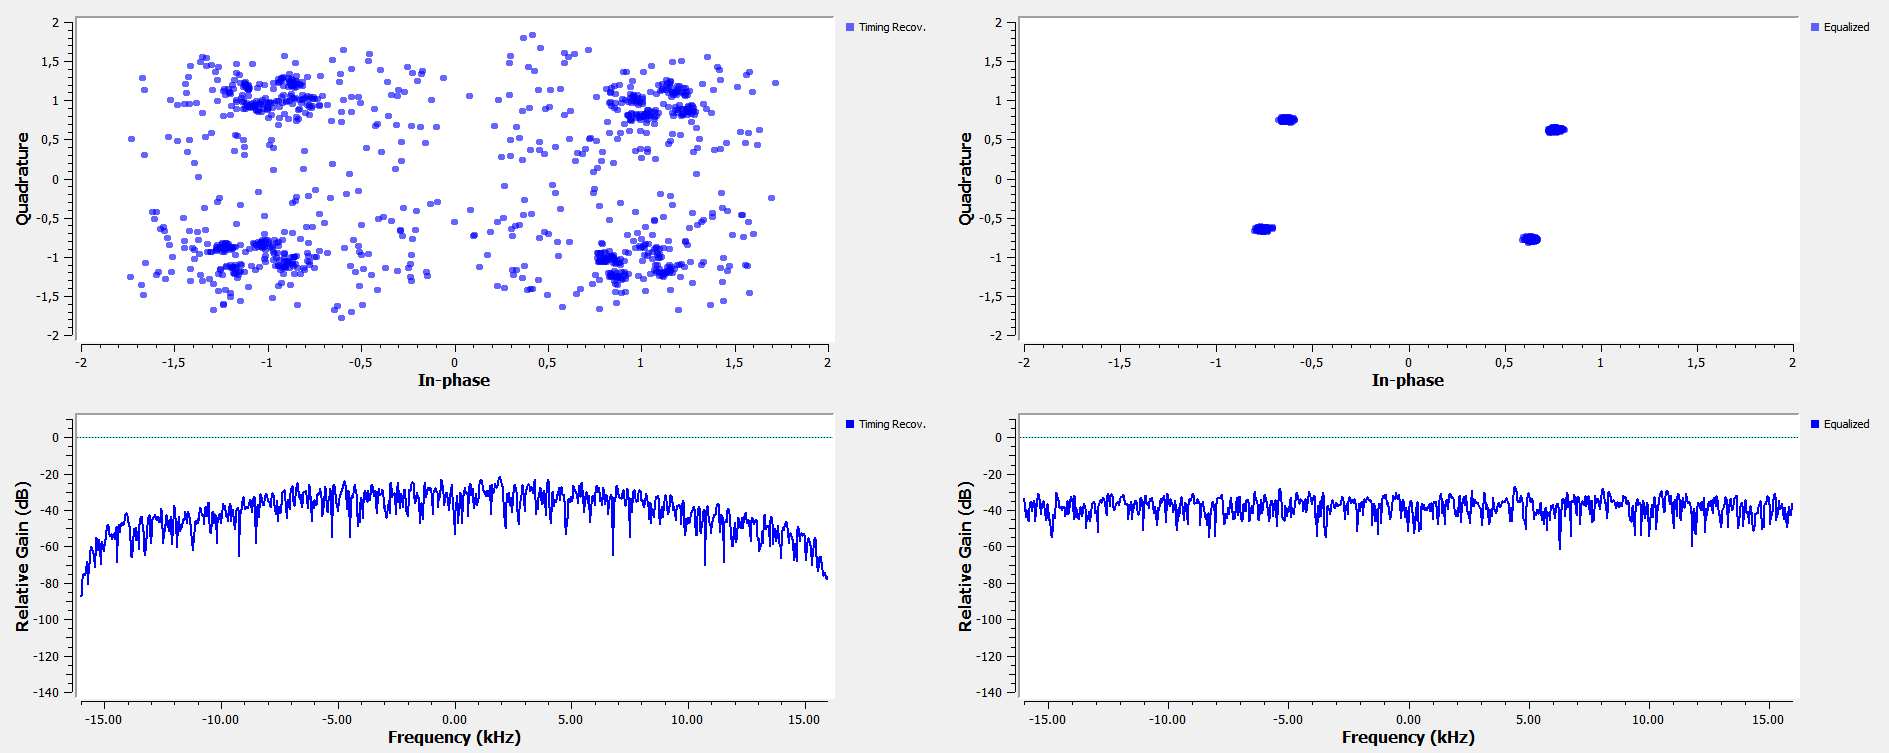
\includegraphics[width=\textwidth]{ex_6_2.png}
                \caption{Результат для \texttt{CMA}}
                \label{fig:ex_6_2}
            \end{figure}
            
            \normalsize{\LARGE \textbf{LMS-DD}}
            
            Задача теперь заключается в использовании блока эквалайзера с наименьшим средним квадратом, направленным на принятие решений (\texttt{LMS-DD}). В отличие слепого эквалайзера, такого как \texttt{CMA}, этот эквалайзер должен знать точки созвездия.
            
            Эквалайзер с наименьшим средним квадратом отлично подходит для сигналов, которые не соответствуют требованиям к постоянному модулю алгоритма \texttt{CMA}, поэтому он может работать с модуляцией типа \texttt{QAM}. С другой стороны, если \texttt{SNR} достаточно плох, принимаемые решения неверны, что может негативно отразиться на производительности приемника. Блок также является более сложным в вычислительном отношении. Данный эквалайзер может производить сигналы лучшего качества, потому что он имеет прямое знание сигнала. Идея состоит в том, чтобы использовать слепой эквалайзер для первоначального сбора, чтобы получить достаточно хороший сигнал, который эквалайзер с наименьшим средним квадратом возьмет на себя.
            
            Был взяn \texttt{mpskstage4.grc} - файл, в котором эквалайзер \texttt{CMA} был заменен на эквалайзер \texttt{LMS-DD}. Этот блок использует объект созвездия, поэтому сложность здесь заключается в создании правильного объекта созвездия для сигнала \texttt{QPSK}.
            
            \begin{figure}[H]
                \centering
                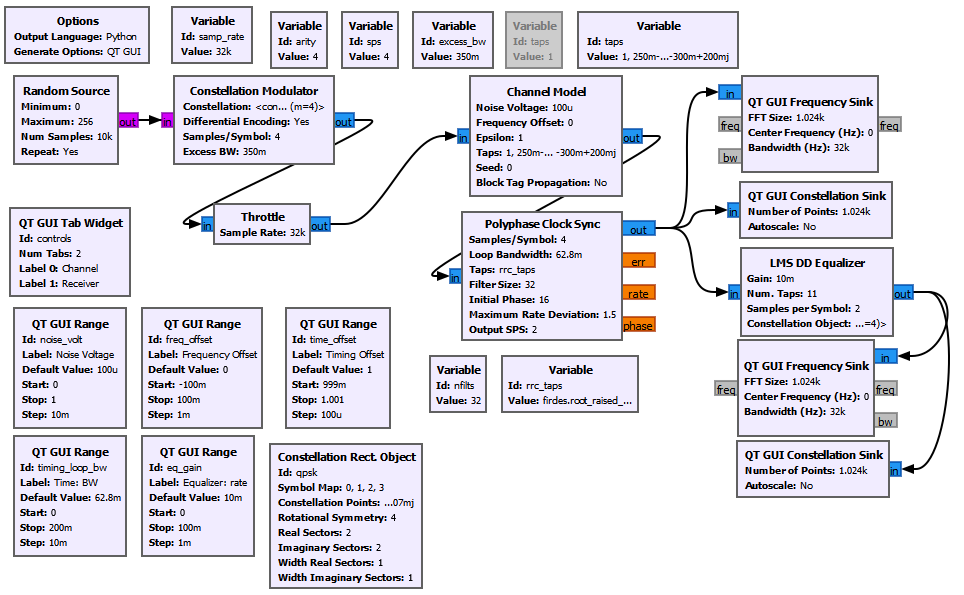
\includegraphics[width=\textwidth]{ex_6_3.png}
                \caption{Эквализация \texttt{LMS}}
                \label{fig:ex_6_3}
            \end{figure}
            
            \begin{figure}[H]
                \centering
                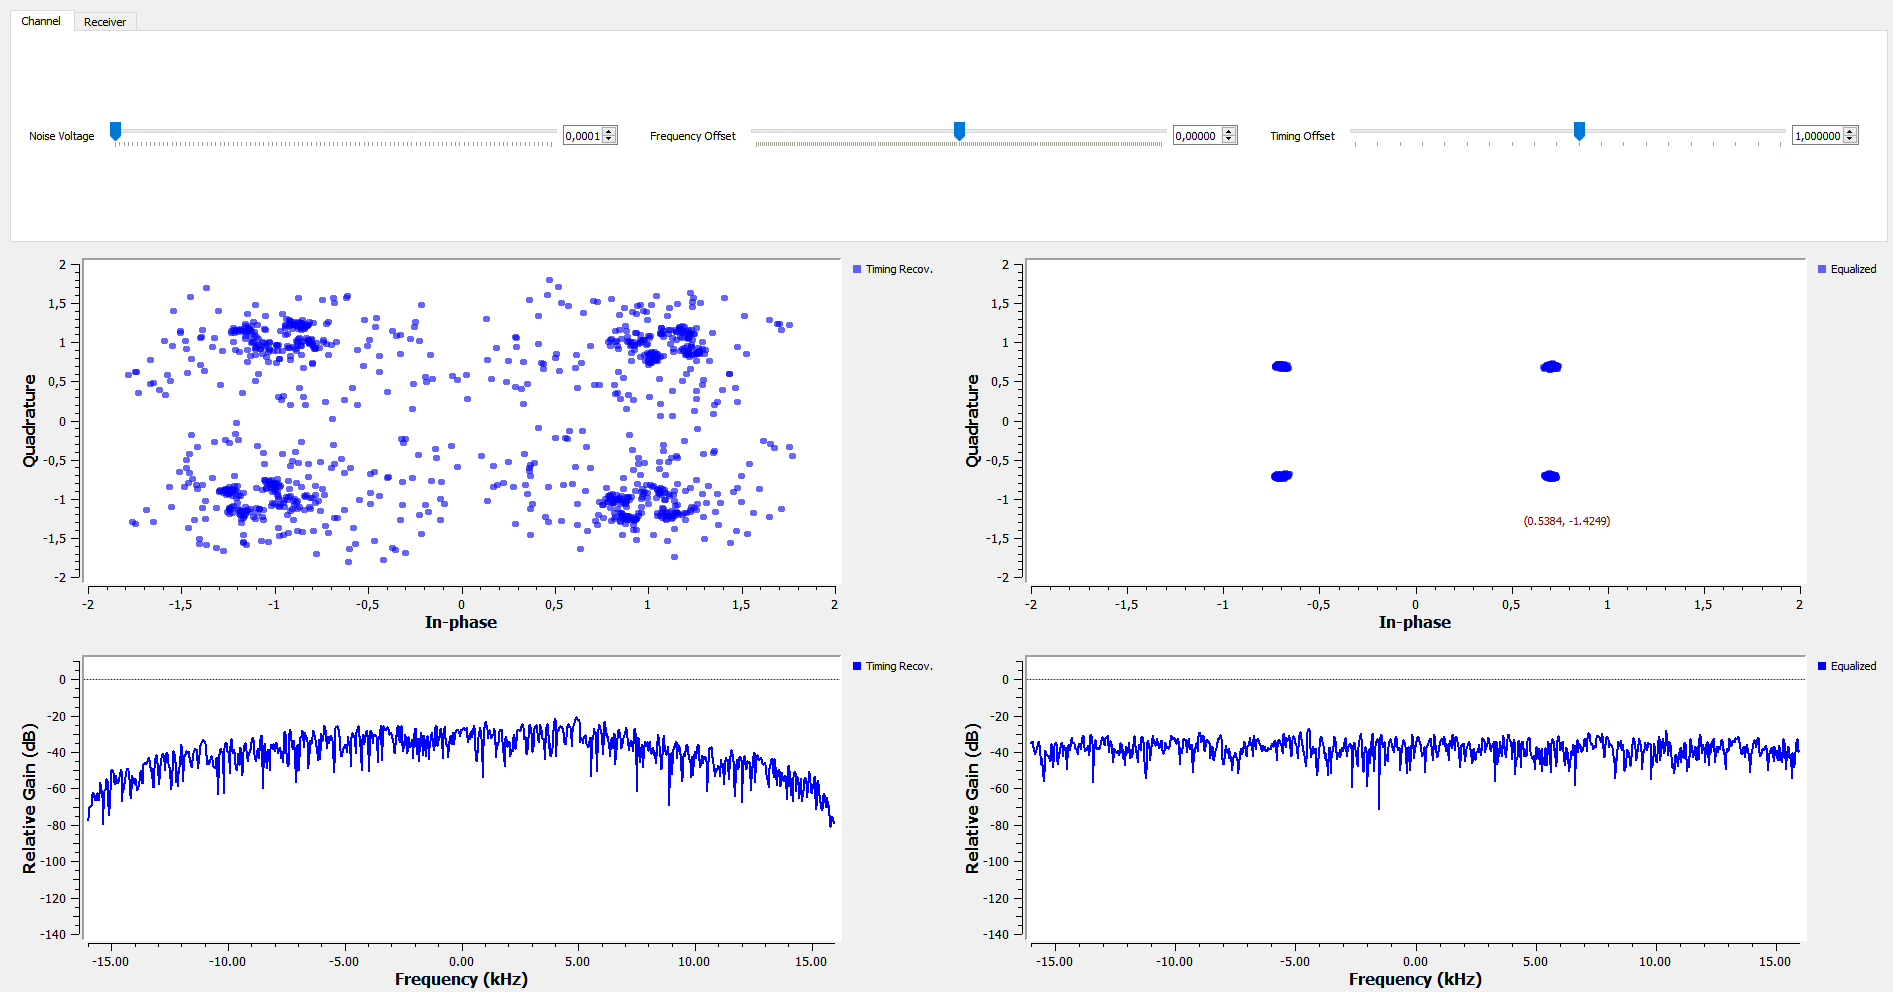
\includegraphics[width=\textwidth]{ex_6_4.png}
                \caption{Результат для \texttt{LMS}}
                \label{fig:ex_6_4}
            \end{figure}
            
            В результате можно сказать, что оба эквалайзера справляются с задачей коррекции искажений, вызванных многолучевым распространением, но \texttt{LMS} эквалайзер к тому же оказывается устойчив к фазовому сдвигу.

    \newpage
        \section{Часть №7: Фазовая и частотная коррекция}
            В седьмом пункте лабораторной работы посмотрим на фазную и частотную корреляцию. Учитывая, что мы выровняли канал, у нас все еще есть проблема смещения фазы и частоты. Эквалайзеры, как правило, не адаптируются быстро, и поэтому могут не успевать за смещением частоты. Кроме того, если просто запустить эквалайзер \texttt{CMA}, достаточным будет являться его схождение к единичному кругу. Он не имеет никакого представления о созвездии, поэтому, когда он блокирует, он будет блокировать в любой заданной фазе. Теперь нужно настроить ситуацию для любого смещения фазы, а также для любого смещения частоты.
            
            Для решения этой проблемы предлагается использовать петлю Костаса. Как и методы, используемые ранее, этот метод использует обратную связь для вычисления ошибки и коррекции фильтра (\texttt{mpskstage5.grc}). Блок петли \texttt{Costas} может синхронизировать \texttt{BPSK}, \texttt{QPSK} и \texttt{8PSK}. Приемник созвездий будет фиксироваться на любом заданном объекте созвездия.
            
            \begin{figure}[H]
                \centering
                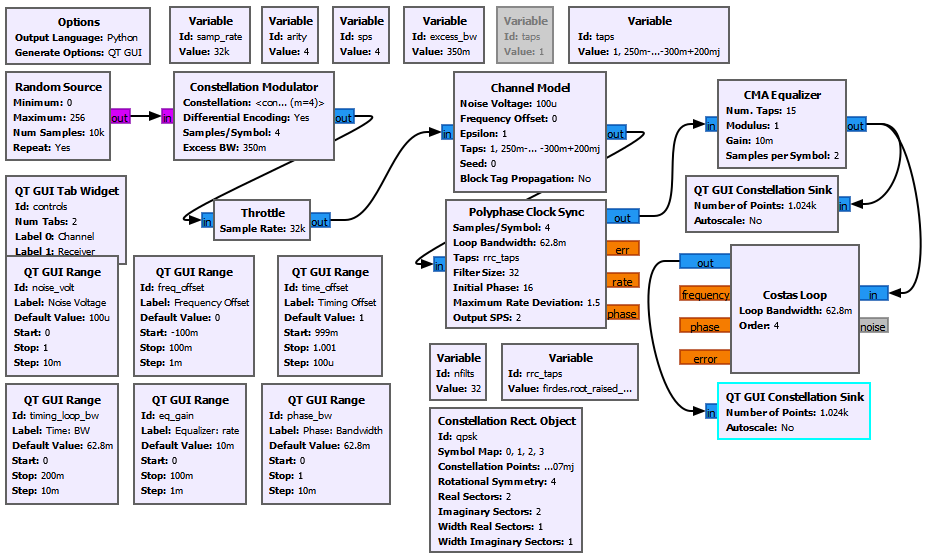
\includegraphics[width=\textwidth]{ex_7_1.png}
                \caption{Фазовая и высокочастотная коррекция}
                \label{fig:ex_7_1}
            \end{figure}
            
            Этот блок, как и все другие, использует цикл второго порядка и поэтому определяется параметром пропускной способности цикла. Другая вещь, которую он должен знать, - это порядок модуляции \texttt{PSK}, поэтому 2 для \texttt{BPSK}, 4 для \texttt{QPSK} и 8 для \texttt{8PSK}. На следующем изображении мы установили шум, смещение времени, простой многолучевой канал и смещение частоты. После эквалайзера мы видим, что все символы находятся на единичном круге, но вращаются из-за смещения частоты, которое еще ничего не исправляет. На выходе блока \texttt{Costas loop} мы можем видеть заблокированное созвездие, как мы начали с него, плюс дополнительный шум, с которым мы ничего не можем поделать.
            
            \begin{figure}[H]
                \centering
                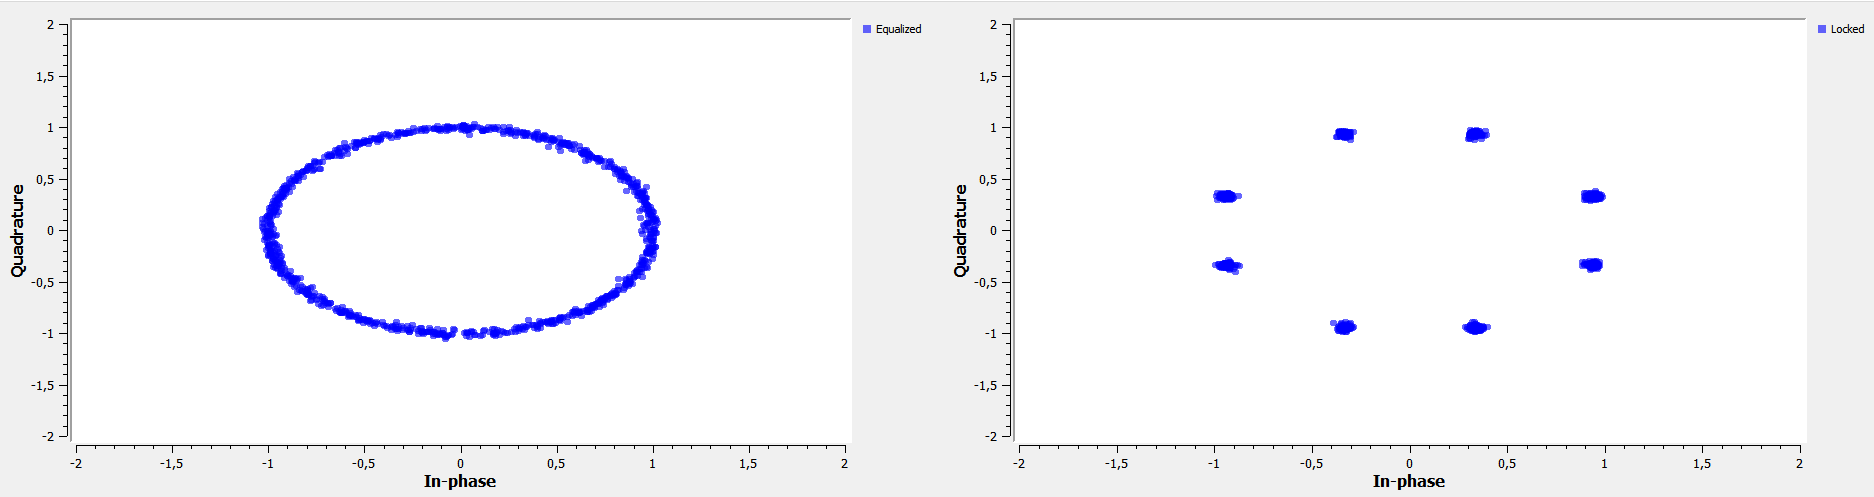
\includegraphics[width=\textwidth]{ex_7_2.png}
                \caption{Первый результат фазовой и высокочастотной коррекции}
                \label{fig:ex_7_2}
            \end{figure}
            
            \begin{figure}[H]
                \centering
                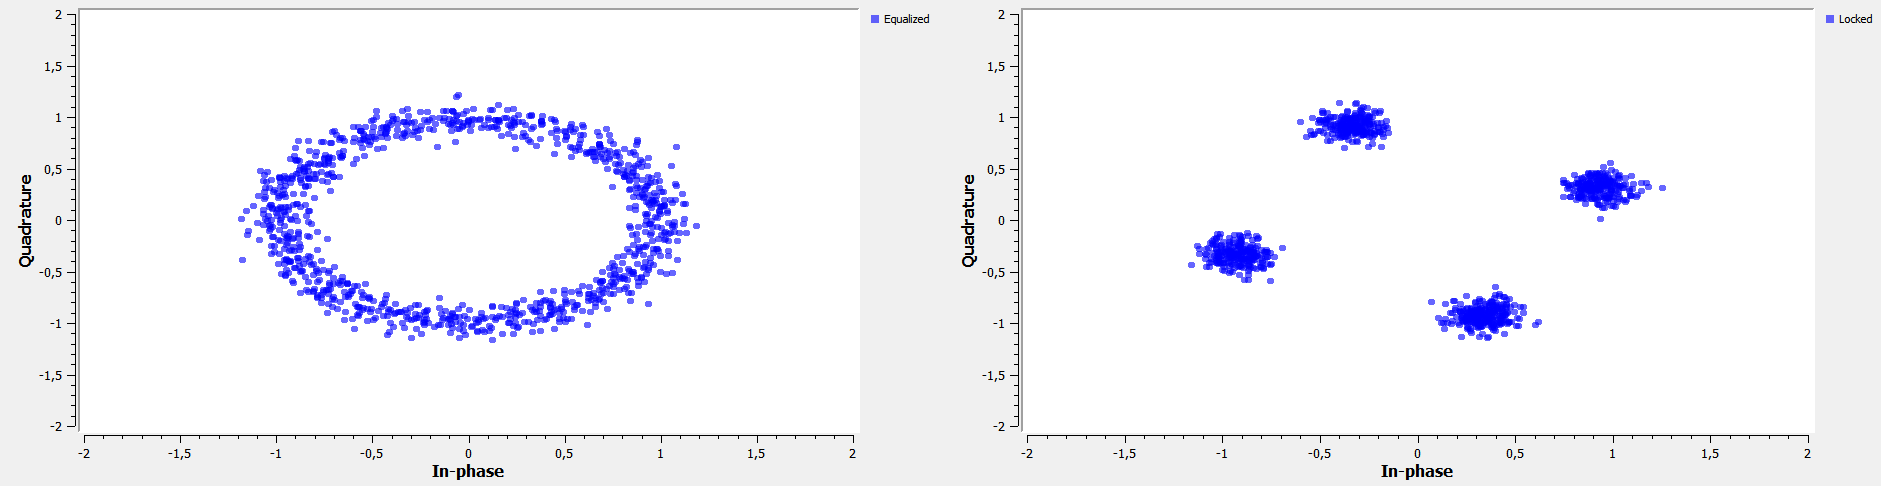
\includegraphics[width=\textwidth]{ex_7_3.png}
                \caption{Результат фазовой и высокочастотной коррекции}
                \label{fig:ex_7_3}
            \end{figure}
            
    \newpage
        \section{Часть №8: Декодирование}
            В заключительном, восьмом пункте лабораторной работы рассмотрим декодирования сигнала. Используя \texttt{mpskstage6.grc} квадратурный демодулятор был установлен после \\\texttt{Costas loop} вместо \texttt{myqpskdemodulator}. В этот момент получены символы от 0 до 3, т. к. это размер алфавита в схеме \texttt{QPSK}. Само созвездие не было фактически передано, вместо этого \\передана разница между его символами, установив дифференциальную настройку в блоке модулятора созвездия как \texttt{True}. 
            
            Чтобы определить, что это исходный байтовый поток, было проведено его сравнение с входным потоко, так как у нас имеется доступ к передаваемым данным при моделировании. 
            
            Использовался блок \texttt{unpack bit} для распаковки от 8-бит на байт до 1-бит на байт. После эти потоки были преобразованы в значения с плавающей точкой 0.0 и 1.0, т. к. временные приемники принимают только плавающие и комплексные значения. Также нам необохдимо задержать передаваемые биты, используя блок \texttt{[[Delay|delay]}.

             \begin{figure}[H]
                \centering
                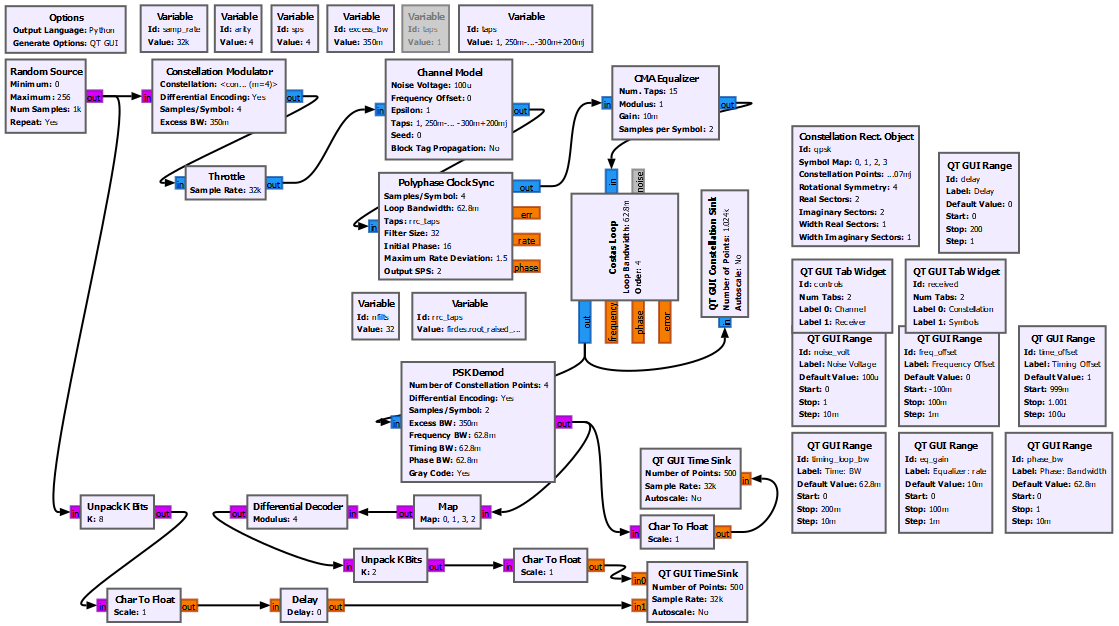
\includegraphics[width=\textwidth]{ex_8_1.png}
                \caption{Передача созвездия \texttt{QPSK}}
                \label{fig:ex_8_1}
            \end{figure}
            
            Чтобы увидеть, когда сигналы синхронизируются, мы можем вычесть один из другого (поскольку выход будет равен 0). Добавление шума и других влияний канала может быть легко замечено как битовые ошибки (когда этот сигнал не равен 0). 
            
            В качестве заключительного эксперимента используется генератор случайных чисел конечной длины, поэтому возможно увидеть шаблон в полученном сигнале. Используя приемник растра времени графического интерфейса \texttt{QT}, он был настроен так, чтобы этот шаблон можно было увидеть.
            
            \begin{figure}[H]
                \centering
                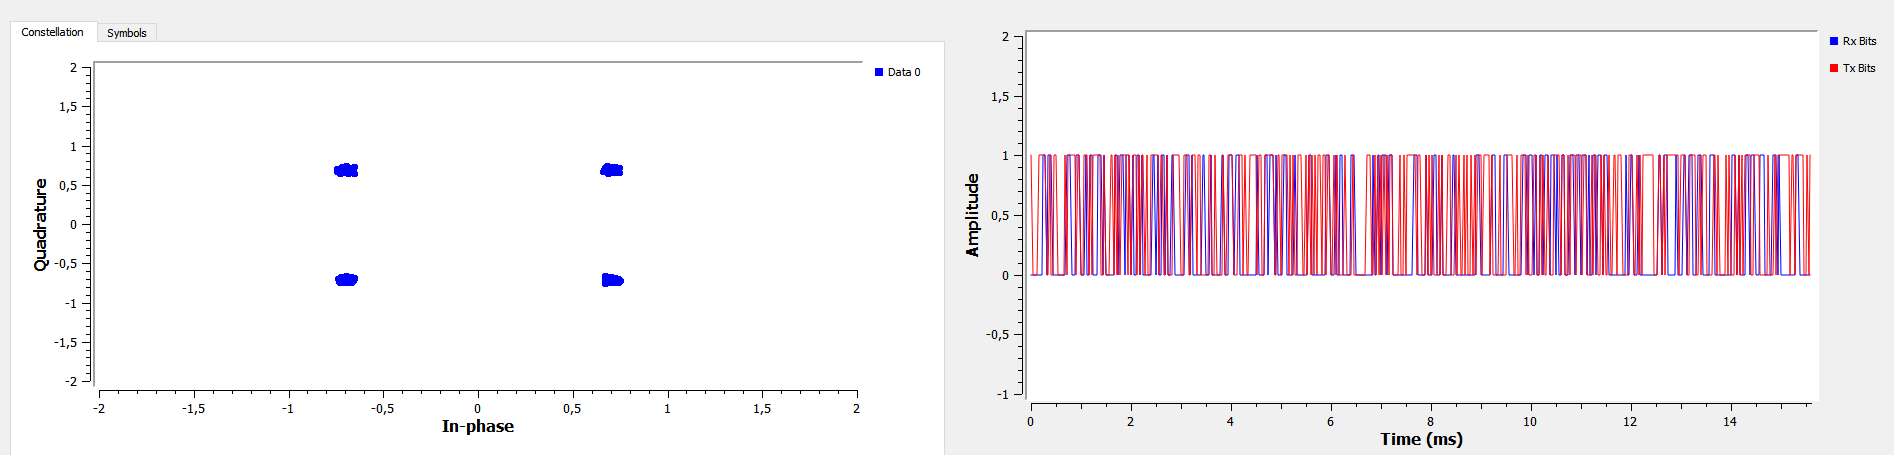
\includegraphics[width=\textwidth]{ex_8_2.png}
                \caption{Вид результата}
                \label{fig:ex_8_2}
            \end{figure}
            
    \newpage
        \section{Выводы}
            В результате выполнения лабораторной работы нами были расмотрены все стадии процесса приема-передачи процесса. Весь процесс был разбит на промежуточные шаги, что позволило лучше разобраться в его работе, участь все факторы, влияющие на передачу, примем и транслирование сигнала.
            
\end{document}
